\begin{singlespace}
    \chapter{\textbf{Optimal resource investment to photosynthetic capacity maximizes nutrient allocation to whole plant growth under elevated CO2}}
\end{singlespace}
    
\section{Introduction}

Terrestrial ecosystems are regulated by complex carbon and nitrogen cycles. As a result, terrestrial biosphere models, which are beginning to include coupled carbon and nitrogen cycles \shortcite{Shi2016,Davies-Barnard2020,Braghiere2022}, must accurately represent these cycles under different environmental scenarios to reliably simulate carbon and nitrogen atmosphere-biosphere fluxes \shortcite{Hungate2003,Prentice2015}. While the inclusion of coupled carbon and nitrogen cycles tends to reduce model uncertainty \shortcite{Arora2020}, large uncertainty in role of soil nitrogen availability and nitrogen acquisition strategy on leaf and whole plant acclimation responses to CO\textsubscript{2} remains \shortcite{Smith2013,Terrer2018,Smith2020}. This source of uncertainty likely contributes to the widespread divergence in future carbon and nitrogen flux simulations across terrestrial biosphere models \shortcite{Friedlingstein2014,Zaehle2014,Meyerholt2020}.

Plants grown under elevated CO\textsubscript{2} generally have less leaf nitrogen content than those grown under ambient CO\textsubscript{2}, a response that often corresponds with reductions in photosynthetic capacity and stomatal conductance at the leaf-level and biomass stimulation over time at the whole plant level \shortcite{Curtis1996,Drake1997,Ainsworth2002,Makino2003,Morgan2004,Ainsworth2005,Ainsworth2007,Smith2013,Poorter2022}. As net primary productivity is generally limited by nitrogen availability \shortcite{Vitousek1991,LeBauer2008,Fay2015}, and soil nitrogen availability is often positively correlated with leaf nitrogen content and photosynthetic capacity \shortcite{Field1986,EvansSeemann1989,Evans1989_photoN,Walker2014,Firn2019,Liang2020}, some have hypothesized that leaf and whole plant acclimation responses to CO\textsubscript{2} are constrained by soil nitrogen availability. The progressive nitrogen limitation hypothesis predicts that elevated CO\textsubscript{2} will increase plant nitrogen demand, which will increase plant nitrogen uptake and progressively deplete soil nitrogen if soil nitrogen supply does not exceed plant nitrogen demand \shortcite{Luo2004}. The hypothesis predicts that this response should result in strong acute stimulations in whole plant growth and primary productivity that diminish over time as nitrogen becomes more limiting. Assuming a positive relationship between soil nitrogen availability, leaf nitrogen content, and photosynthetic capacity, this hypothesis also implies that progressive reductions in soil nitrogen availability should be the mechanism that drives the downregulation in leaf nitrogen content and photosynthetic capacity under elevated CO\textsubscript{2}. This hypothesis has received some support from free air CO\textsubscript{2} enrichment experiments \shortcite{Reich2006,Norby2010}, although is not consistently observed across experiments \shortcite{Finzi2006,Moore2006,Liang2016}.

While possible that progressive nitrogen limitation may determine leaf and whole plant acclimation responses to CO\textsubscript{2}, growing evidence indicates that leaf nitrogen and photosynthetic capacity are more strongly determined through aboveground growing conditions than by soil resource availability \shortcite{Dong2017,Dong2020,Dong2022a,Smith2019,Smith2020,Paillassa2020,Peng2021,Querejeta2022,Westerband2023}, and satellite-derived chlorophyll fluorescence data indicate that increasing atmospheric CO\textsubscript{2} may decrease leaf and canopy demand for nitrogen \shortcite{Dong2022_eCO2}. Together, results from these studies suggest that the downregulation in leaf nitrogen content and photosynthetic capacity due to increasing CO\textsubscript{2} may not be as tightly linked to progressive nitrogen limitation as previously hypothesized.

A unification of optimal coordination and photosynthetic least-cost theories predicts that leaves acclimate to elevated CO\textsubscript{2} by downregulating nitrogen allocation to Ribulose-1,5-bisphosphate (RuBP) carboxylase/oxygenase (Rubisco) to optimize resource use efficiencies at the leaf level, which allows for greater resource allocation to whole plant growth \shortcite{Drake1997,Wright2003,Prentice2014,Smith2019}. The theory predicts that the downregulation in nitrogen allocation to Rubisco results in a stronger downregulation in the maximum rate of Rubisco carboxylation ($V_\mathrm{cmax}$) than the maximum rate of RuBP regeneration ($J_\mathrm{max}$), which maximizes photosynthetic efficiency by allowing net photosynthesis rates to be equally co-limited by Rubisco carboxylation and RuBP regeneration \shortcite{Chen1993,Maire2012}. This acclimation response allows plants to make more efficient use of available light while avoiding overinvestment in Rubisco, which has high nitrogen and energetic costs of building and maintaining \shortcite{Evans1989_photoN,Evans2019}. Instead, additional acquired resources not needed to optimize leaf photosynthesis are allocated to the maintenance of structures that support whole plant growth (e.g., total leaf area, whole plant biomass, etc.) or to allocation processes not related to leaf photosynthesis or growth, such as plant defense mechanisms or leaf structural tissue. Regardless, optimized resource allocation at the leaf level should allow for greater resource allocation to whole plant growth. The theory indicates that leaf acclimation responses to CO\textsubscript{2} should be independent of changes in soil nitrogen availability. While this leaf acclimation response maximizes nitrogen allocation to structures that support whole plant growth, the theory suggests that the positive effect of elevated CO\textsubscript{2} on whole plant growth may be further stimulated by soil nitrogen availability through a reduction in the cost of acquiring nitrogen \shortcite{Bae2015,Perkowski2021,Lu2022}.

Plants acquire nitrogen by allocating photosynthetically derived carbon belowground in exchange for nitrogen through different nitrogen acquisition strategies. These nitrogen acquisition strategies can include direct uptake pathways such as mass flow or diffusion \shortcite{Barber1962}, symbioses with mycorrhizal fungi or symbiotic nitrogen-fixing bacteria \shortcite{Vance1991,Marschner1994,Smith2008,Udvardi2013}, or through the release of root exudates that prime free-living soil microbial communities \shortcite{Phillips2011,Wen2022}. Plants cannot acquire nitrogen without first allocating carbon belowground, which implies an inherent carbon cost to the plant for acquiring nitrogen regardless of nitrogen acquisition strategy. Carbon costs to acquire nitrogen often vary in species with different nitrogen acquisition strategies and are dependent on external environmental factors such as atmospheric CO\textsubscript{2}, light availability, and soil nitrogen availability \shortcite{Brzostek2014FUN2,Terrer2016,Terrer2018,Allen2020,Perkowski2021,Lu2022}, which suggests that acquisition strategy may be an important factor in determining effects of soil nitrogen availability on leaf and whole plant acclimation responses to elevated CO\textsubscript{2}.

A recent meta-analysis using data across 20 grassland and forest CO\textsubscript{2} enrichment experiments suggested that species which acquire nitrogen from symbiotic nitrogen-fixing bacteria had reduced costs of nitrogen acquisition under elevated CO\textsubscript{2} \shortcite{Terrer2018}. Findings from this meta-analysis indicated that reductions in costs of nitrogen acquisition in species that form associations with symbiotic nitrogen-fixing bacteria under elevated CO\textsubscript{2} may drive stronger stimulations in whole plant growth and downregulations in $V_\mathrm{cmax}$ than species that associate with arbuscular mycorrhizal fungi \shortcite{Smith2020}, which generally have higher costs of nitrogen acquisition under elevated CO\textsubscript{2} \shortcite{Terrer2018}. However, plant investments in symbiotic nitrogen fixation generally decline with increasing nitrogen availability \shortcite{Dovrat2018,Perkowski2021}, a response that has been previously inferred to be the result of a shift in the dominant mode of nitrogen acquisition to direct uptake pathways as costs of direct uptake decrease with increasing soil nitrogen availability \shortcite{Rastetter2001,Perkowski2021}. Thus, effects of symbiotic nitrogen fixation on plant acclimation responses to CO\textsubscript{2} should decline with increasing soil nitrogen availability, although manipulative experiments that directly test these patterns are rare.

Here, we conducted a 7-week growth chamber experiment using \textit{Glycine max} L. (Merr.) to examine the effects of soil nitrogen fertilization and inoculation with symbiotic nitrogen-fixing bacteria on leaf and whole plant acclimation responses to elevated CO\textsubscript{2}. Following patterns expected from theory, we hypothesized that individual leaves should acclimate to elevated CO\textsubscript{2} by more strongly downregulating $V_\mathrm{cmax}$ relative to $J_\mathrm{max}$, allowing leaf photosynthesis to approach optimal coordination. We expected this response to correspond with a stronger downregulation in leaf nitrogen content than $V_\mathrm{cmax}$ and $J_\mathrm{max}$, which would increase the fraction of leaf nitrogen content allocated to photosynthesis and photosynthetic nitrogen use efficiency. At the whole-plant level, we hypothesized that plants would acclimate to elevated CO\textsubscript{2} by stimulating whole plant growth and productivity, a response that would be driven by a strong positive response of total leaf area and aboveground biomass to elevated CO\textsubscript{2}. We predicted that leaf acclimation responses to elevated CO\textsubscript{2} would be independent of soil nitrogen fertilization and inoculation with symbiotic nitrogen-fixing bacteria; however, we expected that increasing soil nitrogen fertilization would increase the positive effect of elevated CO\textsubscript{2} on measures of whole plant growth due to a stronger reduction in the cost of acquiring nitrogen under elevated CO\textsubscript{2} with increasing fertilization. We also expected stronger stimulations in whole plant growth due to inoculation, but that this effect would only be apparent under low fertilization due to a reduction in root nodulation with increasing fertilization.

\section{Methods}
\subsection{\textit{Seed treatments and experimental design}}

\textit{Glycine max} L. (Merr) seeds were planted in 144 6-liter surface sterilized pots (NS-600, Nursery Supplies, Orange, CA, USA) containing a steam-sterilized 70:30 v:v mix of Sphagnum peat moss (Premier Horticulture, Quakertown, PA, USA) to sand (Pavestone, subsidiary of Quikrete Companies, Atlanta, GA, USA). Before planting, all \textit{G. max} seeds were surface sterilized in 2\% sodium hypochlorite for 3 minutes, followed by three separate 3-minute washes with ultrapure water (MilliQ 7000; MilliporeSigma, Burlington, MA USA). A subset of surface sterilized seeds were inoculated with Bradyrhizobium japonicum (Verdesian N-Dure\texttrademark\ Soybean, Cary, NC, USA) in a slurry following manufacturer recommendations (3.12 g inoculant and 241 g deionized water per 1 kg seed).
    
Seventy-two pots were randomly planted with surface-sterilized seeds inoculated with \textit{B. japonicum}, while the remaining 72 pots were planted with surface-sterilized uninoculated seeds. Thirty-six pots within each inoculation treatment were randomly placed in one of two atmospheric CO\textsubscript{2} treatments (ambient and 1000 $\mathrm{\mu mol\ mol^{-1}}$ CO\textsubscript{2}). Pots within each unique inoculation-by-CO\textsubscript{2} treatment combination randomly received one of nine soil nitrogen fertilization treatments equivalent to 0, 35, 70, 105, 140, 210, 280, 350, or 630 ppm N. Nitrogen fertilization treatments were created using a modified Hoagland solution \shortcite{Hoagland1950} designed to keep concentrations of other macronutrients and micronutrients equivalent across treatments (Table S1). Pots received the same fertilization treatment throughout the entire duration experiment, which were applied twice per week in 150 mL doses as topical agents to the soil surface throughout the duration of the experiment. This experimental design yielded a fully factorial experiment with four replicates per unique fertilization-by-inoculation-by-CO\textsubscript{2} combination.

\subsection{\textit{Growth chamber conditions}}

Upon experiment initiation, pots were randomly placed in one of six Percival LED-41L2 growth chambers (Percival Scientific Inc., Perry, IA, USA) over two experimental iterations due to chamber space limitation. two iterations were conducted such that one iteration included all elevated CO\textsubscript{2} pots and the second iteration included all ambient CO\textsubscript{2} pots. Average ($\pm$ SD) CO\textsubscript{2} concentrations across chambers throughout the experiment were 439 $\pm$ 5 $\mathrm{\mu mol\ mol^{-1}}$ for the ambient CO\textsubscript{2} treatment and 989 $\pm$ 4 $\mathrm{\mu mol\ mol^{-1}}$ for the elevated CO\textsubscript{2} treatment.
    
Daytime growing conditions were simulated using a 16-hour photoperiod, with incoming light radiation set to chamber maximum (mean $\pm$ SD: 1240 $\pm$ 32 $\mathrm{\mu mol\ m^{-2}\ s^{-1}}$ across chambers), air temperature set to 25\textdegree{}C, and relative humidity set to 50\%. The remaining 8 hours simulated nighttime growing conditions, with incoming light radiation set to 0 $\mathrm{\mu mol\ m^{-2}\ s^{-1}}$, chamber temperature set to 17\textdegree{}C, and relative humidity set to 50\%. Transitions between daytime and nighttime growing conditions were simulated by ramping incoming light radiation in 45-minute increments and temperature in 90-minute increments over a 3-hour period (Table S2).
    
Including the two, 3-hour ramping periods, pots grew under average ($\pm$ SD) daytime light intensity of 1049 $\pm$ 27 $\mathrm{\mu mol\ m^{-2}\ s^{-1}}$. In the elevated CO\textsubscript{2} iteration, pots grew under 24.0 $\pm$ 0.2\textdegree{}C during the day, 16.4 $\pm$ 0.8\textdegree{}C during the night, and 51.6 $\pm$ 0.4\% relative humidity. In the ambient CO\textsubscript{2} iteration, pots grew under 23.9 $\pm$ 0.2\textdegree{}C during the day, 16.0 $\pm$ 1.4\textdegree{}C during the night, and 50.3 $\pm$ 0.2\% relative humidity. We accounted for climatic differences across the six chambers by shuffling the same group of pots daily throughout the growth chambers. This process was done by iteratively moving the group of pots on the top rack of a chamber to the bottom rack of the same chamber, while simultaneously moving the group of pots on the bottom rack of a chamber to the top rack of the adjacent chamber. We moved pots within and across chambers every day throughout the course of each experiment iteration.

\subsection{\textit{Leaf gas exchange measurements}}

Gas exchange measurements were collected for all individuals on the seventh week of development. All gas exchange measurements were collected on the center leaf of the most recent fully expanded trifoliate leaf set. Specifically, we measured net photosynthesis ($A_\mathrm{{net}}$; $\mathrm{\mu mol\ m^{-2}\ s^{-1}}$), stomatal conductance ($g_\mathrm{{sw}}$; $\mathrm{mol\ m^{-2}\ s^{-1}}$), and intercellular CO\textsubscript{2} ($C_\mathrm{{i}}$; $\mathrm{\mu mol\ mol^{-1}}$) concentrations across a range of atmospheric CO\textsubscript{2} concentrations (i.e., an $A_\mathrm{{net}}/C_\mathrm{i}$ curve) using the Dynamic Assimilation Technique\texttrademark. The Dynamic Assimilation Technique\texttrademark\ has been shown to correspond well with traditional steady-state CO\textsubscript{2} response curves in \textit{G. max} \shortcite{Saathoff2021}. $A_\mathrm{{net}}/C_\mathrm{i}$ curves were generated along a reference CO\textsubscript{2} ramp down from 420 $\mathrm{\mu mol\ mol^{-1}}$ CO\textsubscript{2} to 20 $\mathrm{\mu mol\ mol^{-1}}$ CO\textsubscript{2}, followed by a ramp up from 420 $\mathrm{\mu mol\ mol^{-1}}$ CO\textsubscript{2} to 1620 $\mathrm{\mu mol\ mol^{-1}}$ CO\textsubscript{2} after a 90-second wait period at 420 $\mathrm{\mu mol\ mol^{-1}}$ CO\textsubscript{2}. The ramp rate for each curve was set to 200 $\mathrm{\mu mol\ mol^{-1}\ min^{1}}$, logging every five seconds, which generated 96 data points per response curve. All $A_\mathrm{{net}}/C_\mathrm{i}$ curves were generated after $A_\mathrm{{net}}$ and $g_\mathrm{{sw}}$ stabilized in a LI-6800 cuvette set to a 500 $\mathrm{mol\ s^{-1}}$, 10,000 rpm mixing fan speed, 1.5 kPa vapor pressure deficit, 25\textdegree{}C leaf temperature, 2000 $\mathrm{\mu mol\ m^{-2}\ s^{-1}}$ incoming light radiation, and initial reference CO\textsubscript{2} set to 420 $\mathrm{\mu mol\ mol^{-1}}$.

With the same focal leaf used to generate $A_\mathrm{{net}}/C_\mathrm{i}$ curves, we measured dark respiration ($R_\mathrm{{d25}}$; $\mathrm{\mu mol\ m^{-2}\ s^{-1}}$) following at least a 30-minute period of darkness. Measurements were collected on a 5-second log interval for 60 seconds after stabilizing in a LI-6800 cuvette set to a 500 $\mathrm{mol\ s^{-1}}$, 10,000 rpm mixing fan speed, 1.5 kPa vapor pressure deficit, 25\textdegree{}C leaf temperature, and 420 $\mathrm{\mu mol\ mol^{-1}}$ reference CO\textsubscript{2} concentration (for both CO\textsuperscript{2} concentrations), with incoming light radiation set to 0 $\mathrm{\mu mol\ m^{-2}\ s^{-1}}$. A single dark respiration value was determined for each focal leaf by calculating the mean dark respiration value (i.e. the absolute value of $A_\mathrm{{net}}$ during the logging period) across the logging interval.

\subsection{\textit{Leaf trait measurements}}

The focal leaf used to generate $A_\mathrm{{net}}/C_\mathrm{i}$ curves and dark respiration was harvested immediately following gas exchange measurements. Images of each focal leaf were curated using a flat-bed scanner to determine wet leaf area using the 'LeafArea' R package \shortcite{Katabuchi2015}, which automates leaf area calculations using ImageJ software \shortcite{Schneider2012}. Each leaf was dried at 65\textdegree{}C for at least 48 hours, and subsequently weighed and ground until homogenized. Leaf mass per area ($M_\mathrm{area}$; $\mathrm{g\ m^{-2}}$) was calculated as the ratio of dry leaf biomass to fresh leaf area. Using subsamples of ground and homogenized leaf tissue, we measured leaf nitrogen content ($N_\mathrm{mass}$; $\mathrm{g N\ g^{-1}}$) through elemental combustion analysis (Costech-4010, Costech, Inc., Valencia, CA, USA). Leaf nitrogen content per unit leaf area ($N_\mathrm{area}$; $\mathrm{g N\ m^{-2}}$) was calculated by multiplying $N_\mathrm{mass}$ and $M_\mathrm{area}$.

We extracted chlorophyll content from a second leaf in the same trifoliate leaf set as the focal leaf used to generate $A_\mathrm{{net}}/C_\mathrm{i}$ curves. Prior to chlorophyll extraction, we used a cork borer to punch between 3 and 5 0.6 $\mathrm{cm^{2}}$ disks from the leaf. Separate images of each punched leaf and set of leaf disks were curated using a flat-bed scanner to determine wet leaf area, again quantified using the 'LeafArea' R package \shortcite{Katabuchi2015}. The punched leaf was dried and weighed after at least 65\textdegree{}C in the drying oven to determine Marea of the chlorophyll leaf.
    
Leaf disks were shuttled into a test tube containing 10mL dimethyl sulfoxide, vortexed, and incubated at 65\text degree{}C for 120 minutes \shortcite{Barnes1992}. Incubated test tubes were vortexed again before loaded in 150 $\mu$L triplicate aliquots to a 96-well plate. Dimethyl sulfoxide was also loaded in a 150 $\mu$L triplicate aliquot as a blank. Absorbance measurements at 649.1 nm ($A_{649.1}$) and 665.1 nm ($A_{665.1}$) were read in each well using a plate reader (Biotek Synergy H1; Biotek Instruments, Winooski, VT USA) \shortcite{Wellburn1994}, with triplicates subsequently averaged and corrected by the mean of the blank absorbance value. Blank-corrected absorbance values were used to estimate $Chl_\mathrm{a}$ ($\mathrm{\mu g\ mL^{-1}}$) and $Chl_\mathrm{b}$ ($\mathrm{\mu g\ mL^{-1}}$) following equations from \shortciteN{Wellburn1994}:

\begin{equation} \label{eq_5.1}
    Chl_{a}=12.47A_{665.1}-3.62A_{649.1}
\end{equation}
\noindent and
\begin{equation} \label{eq_5.2}
    Chl_{b}=25.06A_{665.1}-6.50A_{649.1}
\end{equation}
    
\noindent $Chl_\mathrm{a}$ and $Chl_\mathrm{b}$ were converted to $\mathrm{mmol\ mL^{-1}}$ using the molar mass of chlorophyll a (893.51 $\mathrm{g\ mol^{-1}}$) and the molar mass of chlorophyll b (907.47 $\mathrm{g\ mol^{-1}}$), then added together to calculate total chlorophyll content in the dimethyl sulfoxide extractant ($\mathrm{mmol\ mL^{-1}}$). Total chlorophyll content was multiplied by the volume of the dimethyl sulfoxide extractant (10 mL) and converted to area-based chlorophyll content by dividing by the total area of the leaf disks ($Chl_\mathrm{area}$; $\mathrm{mmol\ m^{-2}}$). Mass-based chlorophyll content ($Chl_\mathrm{mass}$; $\mathrm{mmol\ g^{-1}}$) was calculated by dividing $Chl_\mathrm{area}$ by the leaf mass per area of the punched leaf.

\subsection{\textit{A/C\textsubscript{i} curve fitting and parameter estimation}}

We fit $A_\mathrm{{net}}/C_\mathrm{i}$ curves of each individual using the ‘fitaci’ function in the ‘plantecophys’ R package \shortcite{Duursma2015}. This function estimates the maximum rate of Rubisco carboxylation $V_{\mathrm{cmax}}$; $\mathrm{\mu mol\ m^{-2}\ s^{-1}}$) and maximum rate of electron transport for RuBP regeneration ($J_{\mathrm{max}}$; $\mathrm{\mu mol\ m^{-2}\ s^{-1}}$) based on the Farquhar biochemical model of C$_{3}$ photosynthesis \shortcite{Farquhar1980}. Triose phosphate utilization (TPU) limitation was included in all curve fits, and all curve fits included measured dark respiration values. As $A_\mathrm{{net}}/C_\mathrm{i}$ curves were generated using a common leaf temperature, curves were fit using Michaelis-Menton coefficients for Rubisco affinity to CO\textsubscript{2} ($K_\mathrm{c}$; $\mathrm{\mu mol\ mol^{-1}}$) and $\mathrm{O_2}$ ($K_\mathrm{o}$; $\mathrm{\mu mol\ mol^{-1}}$), and the CO\textsubscript{2} compensation point ($\Gamma^*$; $\mathrm{\mu mol\ mol^{-1}}$) reported in \shortciteN{Bernacchi2001}. Specifically, $K_\mathrm{c}$ was set to 404.9 $\mathrm{\mu mol\ mol^{-1}}$, $K_\mathrm{o}$ was set to 278.4 $\mathrm{\mu mol\ mol^{-1}}$, and $\Gamma^*$ was set to 42.75 $\mathrm{\mu mol\ mol^{-1}}$. The use of a common leaf temperature across curves and dark respiration measurements also eliminated the need to manually temperature standardize rate estimates. For clarity, we reference $V_{\mathrm{cmax}}$, $J_{\mathrm{max}}$, and $R_{\mathrm{d}}$ estimates throughout the rest of the paper as $V_{\mathrm{cmax25}}$, $J_{\mathrm{max25}}$, and $R_{\mathrm{d25}}$.

\subsection{Stomatal limitation}

We quantified the extent by which stomatal conductance limited photosynthesis (l; unitless) following equations originally described in \shortciteN{Farquhar1982}. Stomatal limitation was calculated as:

\begin{equation} \label{eq_5.3}
    l = 1 - \frac{A_{net}}{A_{mod}}
\end{equation}
\noindent where $A_\mathrm{mod}$ represents the photosynthetic rate where $C_\mathrm{{i}}=C_\mathrm{{a}}$. $A_\mathrm{mod}$ was calculated as:
\begin{equation} \label{eq_5.4}
    A_{mod} = V_{cmax25} - \frac{420 - \Gamma^*}{420 + K_{m}} - R_{d25}
\end{equation}
\noindent $K_\mathrm{m}$ is the Michaelis-Menten coefficient for Rubisco-limited photosynthesis, calculated as:
\begin{equation} \label{eq_5.5}
    K_{m} = K_{c} \cdot \left ( 1 + \frac{O_i}{K_o} \right )
\end{equation}
\noindent where $O_\mathrm{i}$ refers to leaf intercellular O\textsubscript{2} concentrations, set to 210 $\mathrm{\mu mol\ mol^{-1}}$.

\subsection{\textit{Proportion of leaf nitorgen allocated to photosynthesis and structure}}

We used equations from \shortciteN{Niinemets1997} to estimate the proportion of leaf N content allocated to Rubisco bioenergetics, and light harvesting proteins. The proportion of leaf N allocated to Rubisco ($\rho_\mathrm{{rub}}$; $\mathrm{gN\ gN^{-1}}$) was calculated as a function of $V_\mathrm{cmax25}$ and $N_\mathrm{area}$: 
\begin{equation} \label{eqn_5.6}
    \rho_{rubisco}=\frac{V_{cmax25}N_r}{V_{cr}N_{area}}
\end{equation}
\noindent where $N_\mathrm{r}$ is the amount of nitrogen in Rubisco, set to 0.16 $\mathrm{gN\ (gN\ in\ Rubisco)^{-1}}$ and $V_\mathrm{cr}$ is the maximum rate of RuBP carboxylation per unit Rubisco protein, set to 20.5 $\mathrm{\mu mol\ CO_2\ (g\ Rubisco)^{-1}}$. The proportion of leaf nitrogen allocated to bioenergetics ($\mathrm{\rho_{bioe}}$; $\mathrm{gN\ gN^{-1}}$) was similarly calculated as a function of $J_\mathrm{max25}$ and $N_\mathrm{area}$:
\begin{equation} \label{eqn_5.7}
    \rho_{bioe}=\frac{J_{max25}N_b}{J_{mc}N_{area}}
\end{equation}
\noindent where $N_\mathrm{b}$ is the amount of nitrogen in cytochrome f, set to 0.12407 $\mathrm{gN\ (\mu mol}$ $\mathrm{cytochrome\ f)^{-1}}$ assuming a constant 1: 1: 1.2 cytochrome f: ferredoxin NADP reductase: coupling factor molar ratio \shortcite{EvansSeemann1989,Niinemets1997}, and $J_\mathrm{mc}$ is the capacity of electron transport per cytochrome f, set to 156 $\mathrm{\mu mol\ electron\ (\mu mol\ cytochrome\ f)^{-1} s^{-1}}$.

The proportion of leaf nitrogen allocated to light harvesting proteins was calculated as a function of $Chl_\mathrm{{mass}}$ and $N_\mathrm{{mass}}$:
\begin{equation} \label{eqn_5.8}
    \rho_{light}=\frac{Chl_{mass}}{N_{mass}c_{b}}
\end{equation}
\noindent where $c_\mathrm{{b}}$ is the stoichiometry of the light-harvesting chlorophyll complexes of photosystem II, set to 2.75 mmol chlorophyll (gN in chlorophyll)\textsuperscript{-1}. We used the $N_\mathrm{{mass}}$ value of the focal leaf used to generate $A_\mathrm{{net}}/C_\mathrm{i}$ curves instead of the leaf used to extract chlorophyll content, as the two leaves are from the same trifoliate leaf set and are highly correlated with each other (Figure SX).

The proportion of leaf nitrogen content allocated to photosynthetic tissue ($\rho_\mathrm{{photo}}$; $\mathrm{gN\ gN^{-1}}$) was estimated as the sum of $\rho_\mathrm{{rubisco}}$, $\rho_\mathrm{{bioe}}$, and $\rho_\mathrm{{light}}$.

Finally, the proportion of leaf N content allocated to structural tissue ($\rho_\mathrm{{str}}$; $\mathrm{gN\ gN^{-1}}$) was estimated as:
\begin{equation} \label{eqn_5.9}
    \rho_{structure}=\frac{N_{cw}}{N_{area}}
\end{equation}
\noindent where $N_\mathrm{cw}$ is the leaf N content allocated to cell walls ($\mathrm{gN\ m^{-2}}$), calculated as a function of $M_\mathrm{area}$ using an empirical equation from \shortciteN{Onoda2017}:
\begin{equation} \label{eqn_5.10}
    N_{cw}=0.000355*{M_{area}}^{1.39}
\end{equation}

\subsection{\textit{Whole plant traits}}

Seven weeks after experiment initiation and immediately following gas exchange measurements, we harvested all experimental individuals and separated biomass of each experimental individual into major organ types (leaves, stems, roots, and nodules when present). Fresh leaf area of all harvested leaves was measured using an LI-3100C (Li-COR Biosciences, Lincoln, Nebraska, USA). Total fresh leaf area (cm\textsuperscript{2}) was calculated as the sum of all leaf areas, including the focal leaf used to collect gas exchange data and the focal leaf used to extract chlorophyll content. All harvested material was dried in an oven set to 65\textdegree{}C for at least 48 hours, weighed, and ground to homogeneity. Leaves and nodules were manually ground either with a mortar and pestle, while stems and roots were ground using a Wiley mill (E3300 Mini Mill; Eberbach Corp., MI, USA). Total dry biomass (g) was calculated as the sum of dry leaf (including focal leaf for both the $A_\mathrm{{net}}/C_\mathrm{i}$ curve and leaf used to extract chlorophyll content), stem, root, and root nodule biomass. We also quantified carbon and nitrogen content of each respective organ type through elemental combustion (Costech-4010, Costech, Inc., Valencia, CA, USA) using subsamples of ground and homogenized organ tissue.

Following the approach explained in \shortciteN{Perkowski2021}, we calculated structural carbon costs to acquire nitrogen as the ratio of total belowground carbon biomass to whole plant nitrogen biomass ($N_\mathrm{cost}$; $\mathrm{gC\ gN^{-1}}$). Belowground carbon biomass ($C_\mathrm{bg}$; gC) was calculated as the sum of root carbon biomass and root nodule carbon biomass. Root carbon biomass and root nodule carbon biomass was calculated as the product of the organ biomass and the respective organ carbon content. Whole plant nitrogen biomass ($N_\mathrm{wp}$; gN) was similarly calculated as the sum of total leaf, stem, root, and root nodule nitrogen biomass, including the focal leaf used for $A_\mathrm{{net}}/C_\mathrm{i}$ curve and chlorophyll extractions. Leaf, stem, root, and root nodule nitrogen biomass was calculated as the product of the organ biomass and the respective organ nitrogen content. This calculation only quantifies plant structural carbon costs to acquire nitrogen and does not include any additional costs of nitrogen acquisition associated with respiration, root exudation, or root turnover. An explicit explanation of the limitations for interpreting this calculation can be found in \shortciteN{Perkowski2021} and \shortciteN{Terrer2018}.

Finally, plant investments in nitrogen fixation were calculated as the ratio of root nodule biomass to root biomass, where increasing values indicate an increase in plant investments to nitrogen fixation \shortcite{Dovrat2018,Dovrat2020,Perkowski2021}. We also calculated the percent of leaf nitrogen acquired from the atmosphere (\%$N_\mathrm{dfa}$) using leaf $\delta\mathrm{^{15}{N}}$ and the following equation from \shortciteN{Andrews2011}:

\begin{equation} \label{eqn_5.11}
    \%N_{dfa} = \frac{\delta^{15}N{}_{reference} - \delta^{15}N{}_{sample}}{\delta^{15}N{}_{reference} - B}
\end{equation}
    
\noindent where $\delta\mathrm{^{15}{N}_{reference}}$ refers to a reference plant that exclusively acquires nitrogen via direct uptake, $\delta\mathrm{^{15}{N}_{sample}}$ refers to an individual’s leaf $\delta\mathrm{^{15}{N}}$, and B refers to individuals that are entirely reliant on nitrogen fixation. Within each unique nitrogen fertilization treatment-by-CO\textsubscript{2} treatment combination, we calculated the mean leaf $\delta\mathrm{^{15}{N}}$ for individuals growing in the non-inoculated treatment for $\delta\mathrm{^{15}{N}_{reference}}$. Any individuals with visual confirmation of root nodule formation or nodule initiation were omitted from the calculation of $\delta\mathrm{^{15}{N}_{reference}}$. Following recommendations from Andrews et al. (2011) we calculated B within each CO2 treatment using the mean leaf $\delta\mathrm{^{15}{N}}$ of inoculated individuals that received 0 ppm N. We did not calculate B within each unique soil nitrogen x CO2 treatment combination, as previous studies suggest decreased reliance on nitrogen fixation with increasing soil nitrogen availability \shortcite{Perkowski2021}. This approach for estimating nitrogen fixation standardizes values such that approaching 1 indicates increasing reliance on nitrogen fixation.


\subsection{\textit{Statistical analyses}}
Any uninoculated pots that had substantial root nodule formation (nodule biomass: root biomass values greater than 0.05 $\mathrm{g\ g^{-1}}$) were removed from our analyses. This was because they were assumed to have been colonized by symbiotic nitrogen-fixing bacteria from outside sources. This decision resulted in the removal of sixteen pots from our analysis: two pots in the elevated CO\textsubscript{2} treatment that received 35 ppm N, three pots in the elevated CO\textsubscript{2} treatment that received 70 ppm N, one pot in the elevated CO\textsubscript{2} treatment that received 210 ppm N, two pots in the elevated CO\textsubscript{2} treatment that received 280 ppm N, two pots in the ambient CO\textsubscript{2} treatment that received 0 ppm N, three pots in the ambient CO\textsubscript{2} treatment that received 70 ppm N, two pots in the ambient CO\textsubscript{2} treatment that received 105 ppm N, and one pot in the ambient CO\textsubscript{2} treatment that received 280 ppm N.

We built a series of linear mixed effects models to investigate the impacts of CO\textsubscript{2} concentration, soil nitrogen fertilization, and inoculation with \textit{B. japonicum} on \textit{G. max} gas exchange, tradeoffs between nitrogen and water use, whole plant growth, and investment in nitrogen fixation. All models included CO\textsubscript{2} treatment as a categorical fixed effect, inoculation treatment as a categorical fixed effect, soil nitrogen fertilization as a continuous fixed effect, with interaction terms between all three fixed effects. All models also accounted for climatic difference between chambers across experiment iterations by including a random intercept term that nested starting chamber rack by CO\textsubscript{2} treatment. Models with this independent variable structure were created for each of the following dependent variables: $N_\mathrm{area}$, $M_\mathrm{area}$, $N_\mathrm{mass}$, $Chl_\mathrm{area}$, $V_\mathrm{cmax25}$, $J_\mathrm{max25}$, $J_\mathrm{max25}$:$V_\mathrm{cmax25}$, $R_\mathrm{d25}$, $g_\mathrm{sw}$, stomatal limitation, $\rho_\mathrm{rubisco}$, $\rho_\mathrm{bioe}$, $\rho_\mathrm{light}$, $\rho_\mathrm{photo}$, $\rho_\mathrm{structure}$, $N_\mathrm{cost}$, $C_\mathrm{bg}$, $N_\mathrm{wp}$, total biomass, total leaf area, nodule biomass, and the ratio of nodule biomass to root biomass.

We used Shapiro-Wilk tests of normality to determine whether linear mixed effects models satisfied residual normality assumptions. If residual normality assumptions were not met (Shapiro-Wilk: \textit{p} < 0.05), then models were fit using dependent variables that were natural log transformed. All residual normality assumptions that did not originally satisfy residual normality assumptions were met with either a natural log or square root data transformation (Shapiro-Wilk: \textit{p} > 0.05 in all cases). Specifically, models for $N_\mathrm{area}$, $N_\mathrm{mass}$, $Chl_\mathrm{area}$, $V_\mathrm{cmax25}$, $J_\mathrm{max25}$, $J_\mathrm{max25}$:$V_\mathrm{cmax25}$, $g_\mathrm{sw}$, stomatal limitation, $\rho_\mathrm{rubisco}$, $\rho_\mathrm{bioe}$, $\rho_\mathrm{light}$, $\rho_\mathrm{photo}$, and total leaf area satisfied residual normality assumptions without data transformation. Models for $M_\mathrm{area}$, $\rho_\mathrm{structure}$, $N_\mathrm{cost}$, $C_\mathrm{bg}$, $N_\mathrm{wp}$, and total biomass satisfied residual normality assumptions with a natural log data transformation, while models for nodule biomass and nodule biomass: root biomass satisfied residual normality assumptions with a square root data transformation.

In all statistical models, we used the 'lmer' function in the 'lme4' R package \shortcite{Bates2015} to fit each model and the 'Anova' function in the 'car' R package \shortcite{Fox2019} to calculate Type II Wald's $\chi^{2}$ and determine the significance ($\alpha$ = 0.05) of each fixed effect coefficient. We then used the 'emmeans' R package \shortcite{Lenth2019} to conduct post-hoc comparisons using Tukey's tests, where degrees of freedom were approximated using the Kenward-Roger approach \shortcite{Kenward1997}. All analyses and plots were conducted in R version 4.2.0 \shortcite{RCoreTeam2021}.

\section{Results}
\subsection{\textit{Leaf nitrogen content, chlorophyll content, and mass per area}}

Elevated CO$_2$ reduced $N_\mathrm{area}$, $N_\mathrm{mass}$, and $Chl_\mathrm{area}$ by 29\%, 50\%, and 31\%, respectively, and stimulated $M_\mathrm{area}$ by 44\% (\textit{p} < 0.001 in all cases; Table 1). An interaction between fertilization and CO$_2$ (CO$_2$-by-fertilization interaction: $p_{N\mathrm{area}}$ = 0.017, $p_{N\mathrm{mass}}$ < 0.001, $p_{M\mathrm{area}}$ = 0.006, $p_{Chl\mathrm{area}}$ = 0.083; Table 1) indicated that the general positive effect of increasing fertilization on $N_\mathrm{area}$, $N_\mathrm{mass}$, and $Chl_\mathrm{area}$ (\textit{p} < 0.001 in all cases; Table 1) was generally stronger under ambient CO$_2$ (Tukey$_{N\mathrm{area}}$: \textit{p} = 0.026; Tukey$_{N\mathrm{mass}}$: \textit{p} < 0.001; Tukey$_{M\mathrm{area}}$: \textit{p} = 0.009; Tukey$_{Chl\mathrm{area}}$: \textit{p} = 0.065; Table 1; Figs. 1a-d). This pattern resulted in a stronger reduction in $N_\mathrm{area}$, $N_\mathrm{mass}$, and $Chl_\mathrm{area}$  as well as a stronger stimulation in $M_\mathrm{area}$ under elevated CO$_2$ with increasing fertilization. An additional interaction between inoculation and CO$_2$ on $N_\mathrm{area}$ (CO$_2$-by-inoculation interaction: \textit{p} = 0.030; Table 1) indicated that the general positive effect of inoculation on $N_\mathrm{area}$ (\textit{p} < 0.001; Table 1) was stronger under elevated CO$_2$ (45\% increase; Tukey: \textit{p} < 0.001) than under ambient CO$_2$ (18\% increase; Tukey: \textit{p} < 0.001), a result that increased the reduction in $N_\mathrm{area}$ in inoculated pots under elevated CO$_2$. Inoculation treatment did not modify the downregulation in $N_\mathrm{mass}$ (CO$_2$-by-inoculation interaction: \textit{p} = 0.148; Table 1) and $Chl_\mathrm{area}$ (\textit{p} = 0.147; Table 1) or the stimulation in $M_\mathrm{area}$ (\textit{p} = 0.866; Table 1) under elevated CO$_2$. However, interactions between fertilization and inoculation on $N_\mathrm{area}$ (fertilization-by-inoculation interaction: \textit{p} < 0.001; Table 1; Fig. 1a), $N_\mathrm{mass}$ (\textit{p} = 0.001; Table 1; Fig. 1b), $M_\mathrm{area}$ (\textit{p} = 0.025; Table 1; Fig. 1c), and $Chl_\mathrm{area}$ (\textit{p} < 0.001; Table 1; Fig. 1d) indicated that the general positive effect of increasing fertilization on each trait was stronger in uninoculated pots (Tukey$_{N\mathrm{area}}$: \textit{p} < 0.001; Tukey$_{N\mathrm{mass}}$: \textit{p} = 0.001; Tukey$_{M\mathrm{area}}$: \textit{p} = 0.031; Tukey$_{Chl\mathrm{area}}$: \textit{p} < 0.001).


\newpage
placeholder Table 1
\clearpage

\newpage
\begin{landscape}
    \begin{figure}
        \centering
        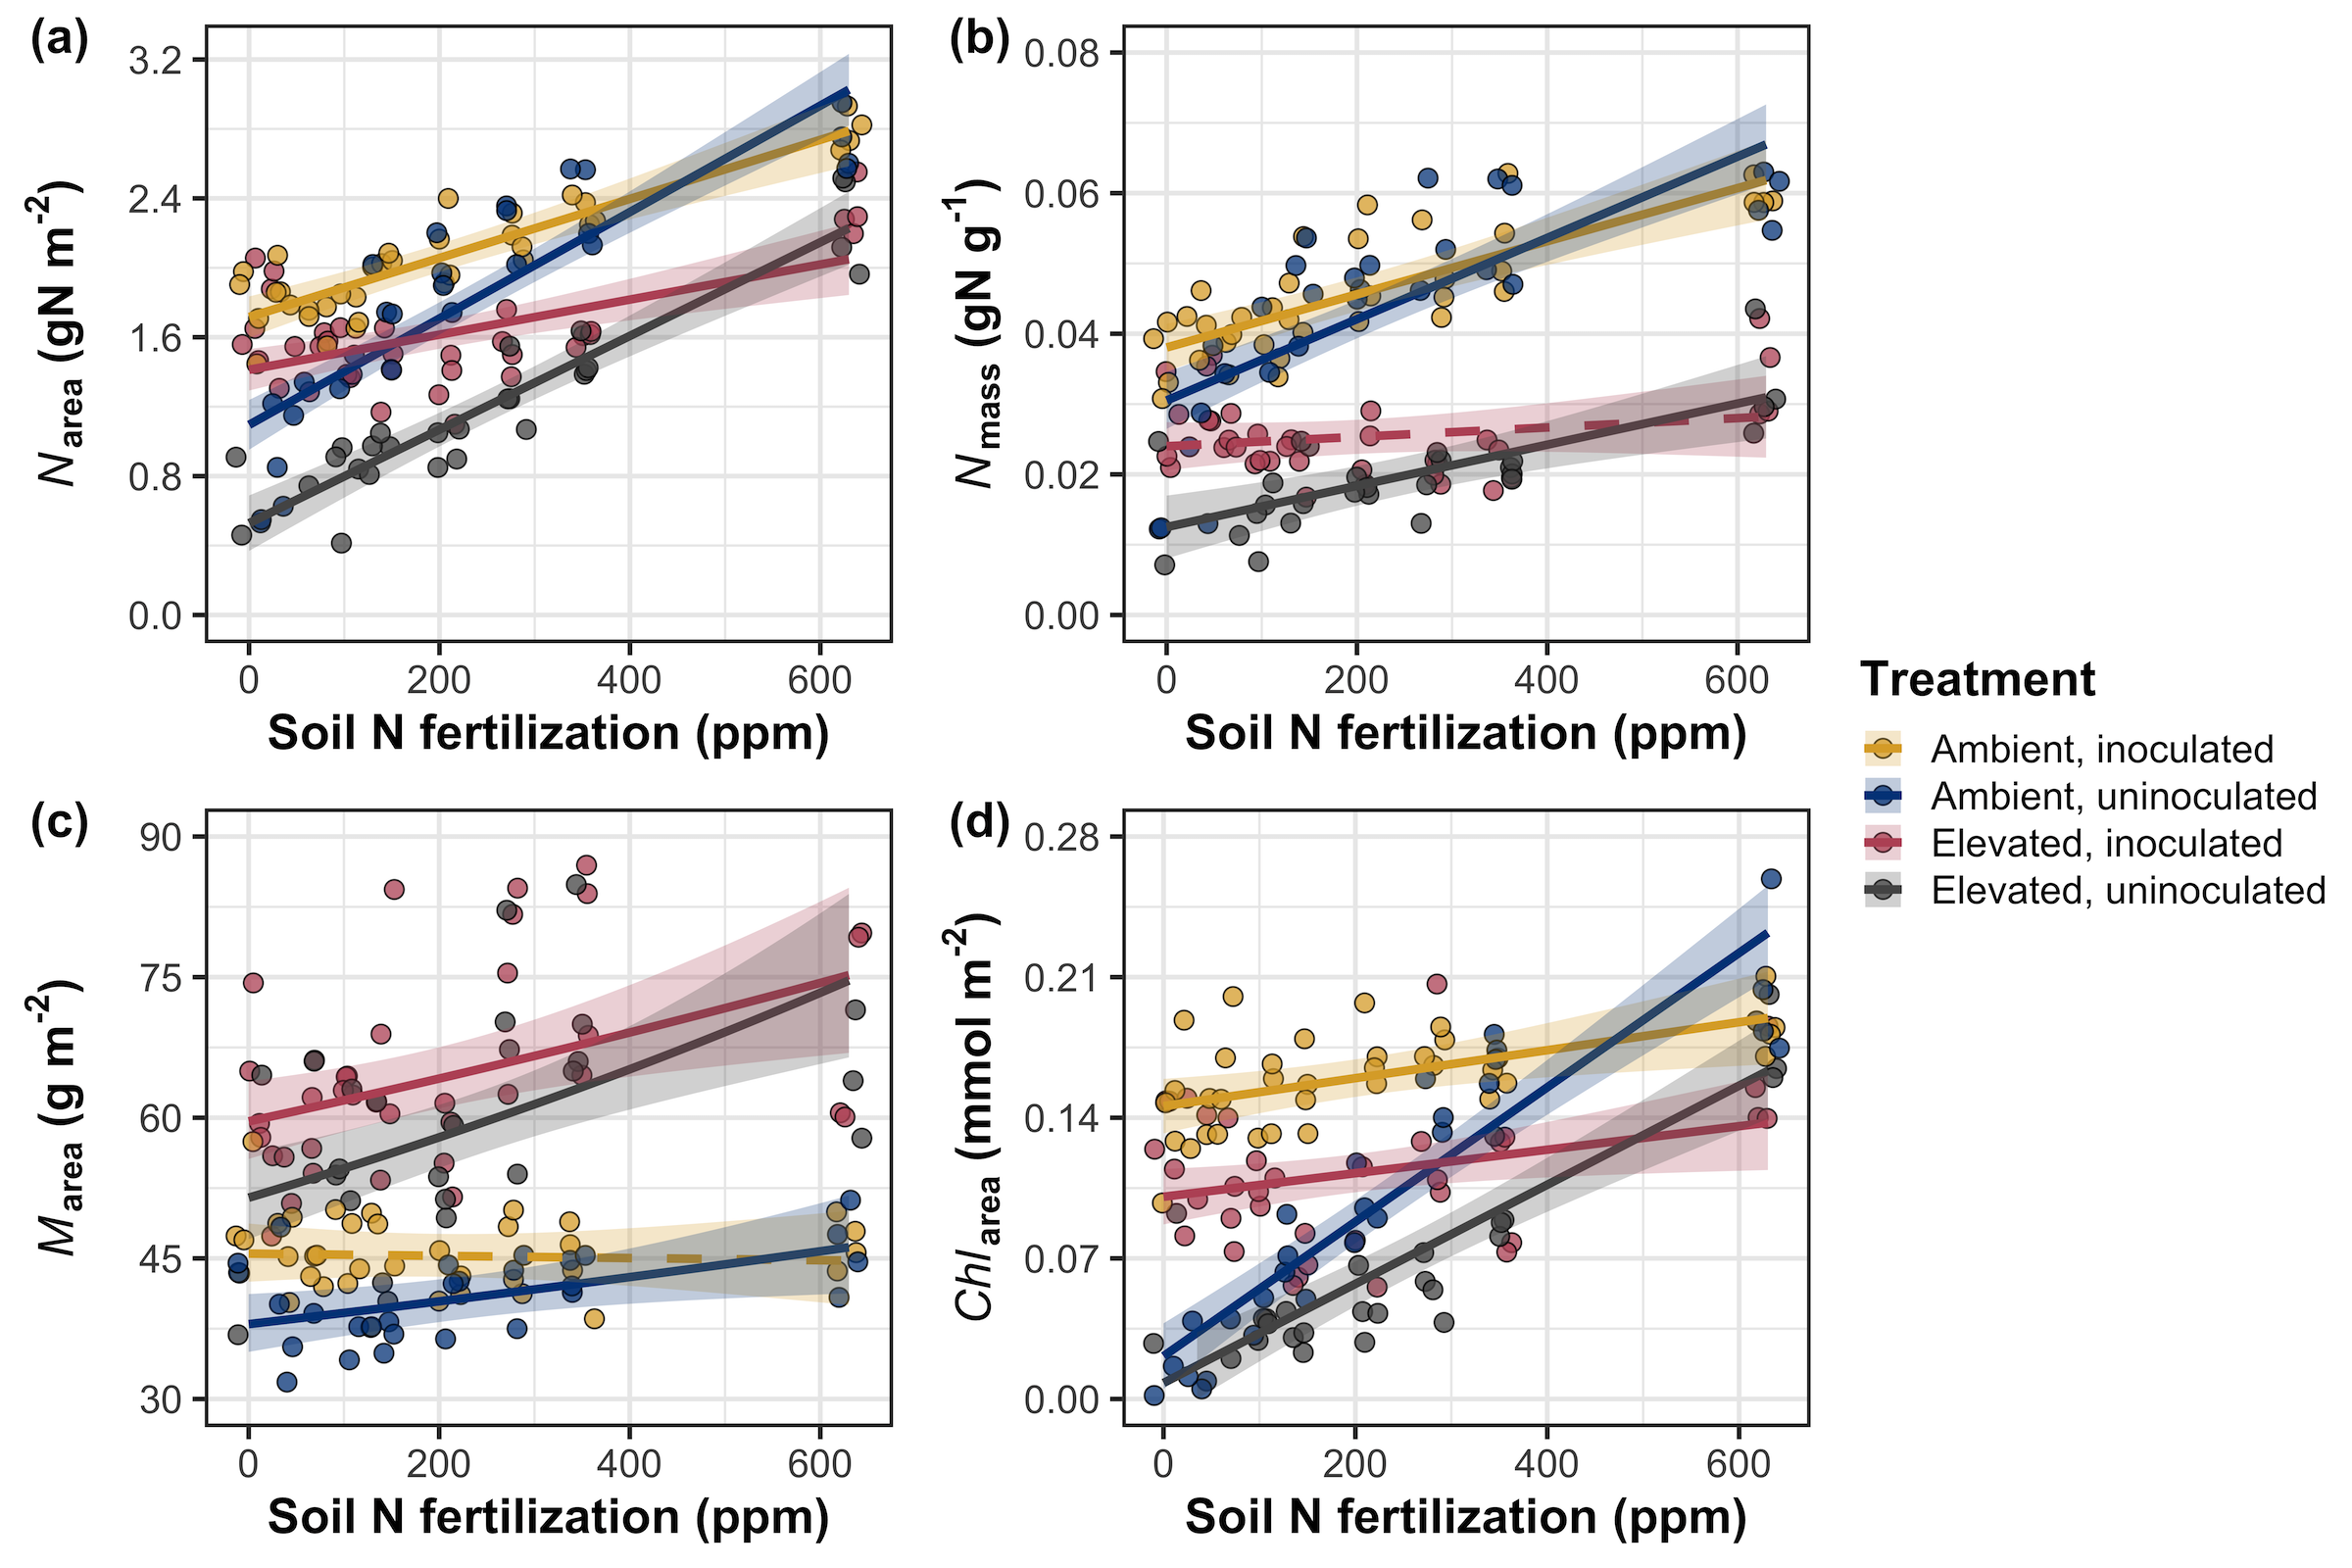
\includegraphics[scale = 0.0625]{ch5_NxCO2xI/figs/NxCO2xI_fig1_leafN.png}
        \caption[Effects of CO$_2$, fertilization, and inoculation on leaf nitrogen per unit leaf area, leaf nitrogen content, leaf mass per unit leaf area, and chlorophyll content per unit leaf area.]{Effects of CO$_2$, fertilization, and inoculation on leaf nitrogen per unit leaf area (a), leaf nitrogen content (b), leaf mass per unit leaf area (c), and chlorophyll content per unit leaf area (d). Soil nitrogen fertilization is represented on the x-axis in all panels. Yellow points and trendlines indicate inoculated individuals grown under ambient CO$_2$, blue points and trendlines indicate uninoculated individuals grown under ambient CO$_2$, red points and trendlines indicate inoculated individuals grown under elevated CO2, and grey points indicate uninoculated individuals grown under elevated CO$_2$. Solid trendlines indicate regression slopes that are different from zero (\textit{p} < 0.05), while dashed trendlines indicate slopes that are not distinguishable from zero (\textit{p} > 0.05).}
        \label{fig:figure5.1}
    \end{figure}
\end{landscape}
\clearpage

\subsection{\textit{Leaf biochemistry and stomatal conductance}}
Elevated CO$_2$ resulted in plants with 16\% lower $V_\mathrm{cmax25}$ (\textit{p} < 0.001; Table 2) and 10\% lower $J_\mathrm{max25}$ (\textit{p} = 0.014; Table 2) as compared to those grown under ambient CO$_2$, but did not influence $R_\mathrm{d25}$ (\textit{p} = 0.613; Table 2). A relatively stronger downregulation in $V_\mathrm{cmax25}$ than $J_\mathrm{max25}$ resulted in an 8\% stimulation in $J_\mathrm{max25}$:$V_\mathrm{cmax25}$ under elevated CO$_2$ (\textit{p} < 0.001; Table 2; Fig. 2E). The downregulatory effect of CO$_2$ on $V_\mathrm{cmax25}$ and $J_\mathrm{max25}$ was not modified across the fertilization gradient (CO$_2$-by-fertilization interaction: \textit{p} = 0.185, \textit{p} = 0.389 for $V_\mathrm{cmax25}$ and $J_\mathrm{max25}$, respectively; Table 2; Fig. 2A, 2C) or between inoculation treatments (CO$_2$-by-inoculation interaction: \textit{p} = 0.799 and \textit{p} = 0.714 for $V_\mathrm{cmax25}$ and $J_\mathrm{max25}$, respectively; Table 2). However, a strong interaction between fertilization and inoculation (fertilization-by-inoculation interaction: p $\le$ 0.001 in all cases; Table 2) indicated that the general positive effect of increasing fertilization on $V_\mathrm{cmax25}$ (\textit{p} < 0.001; Table 2), $J_\mathrm{max25}$ (\textit{p} < 0.001; Table 2), and $R_\mathrm{d25}$ (\textit{p} = 0.015; Table 2) was only observed in uninoculated pots (Tukey: \textit{p} $\le$ 0.001 in all cases), as there was no apparent effect of fertilization on $V_\mathrm{cmax25}$ (Tukey: \textit{p} = 0.456), $J_\mathrm{max25}$ (Tukey: \textit{p} = 0.180), or $R_\mathrm{d25}$ (Tukey: \textit{p} = 0.443) in inoculated pots (Figs. 2B, 2D, 2F, 2H). A relatively stronger positive effect of increasing fertilization on $V_\mathrm{cmax25}$ than $J_\mathrm{max25}$ resulted in a general reduction in $J_\mathrm{max25}$:$V_\mathrm{cmax25}$ with increasing fertilization (\textit{p} < 0.001), though this pattern was only seen in uninoculated pots (Tukey: \textit{p} = 0.003) and not inoculated plants (Tukey: \textit{p} > 0.05).

Elevated CO$_2$ reduced stomatal conductance by 20\% (\textit{p} < 0.001; Table 2) compared to ambient CO$_2$, but this downregulation did not influence stomatal limitation of photosynthesis (\textit{p} = 0.355; Table 2). As with $V_\mathrm{cmax25}$ and $J_\mathrm{max25}$, the downregulation of stomatal conductance due to elevated CO$_2$ was not modified across the fertilization gradient (CO$_2$-by-fertilization interaction: \textit{p} = 0.141; Table 2) or between inoculation treatments (CO$_2$-by-inoculation interaction: \textit{p} = 0.179; Table 2). Fertilization also did not modify the general null effect of CO$_2$ on stomatal limitation (CO$_2$-by-fertilization interaction: \textit{p} = 0.554; Table 2), although an interaction between CO$_2$ and inoculation (CO$_2$-by-inoculation interaction: \textit{p} = 0.043; Table 2) indicated that inoculation increased stomatal limitation under ambient CO$_2$ (Tukey: \textit{p} = 0.021), but not under elevated CO$_2$ (Tukey: \textit{p} > 0.999). An interaction between inoculation and fertilization on stomatal conductance (fertilization-by-inoculation interaction: \textit{p} < 0.001; Table 2) indicated that increasing fertilization increased stomatal conductance in uninoculated pots (Tukey: \textit{p} = 0.003) but decreased stomatal conductance in inoculated pots (Tukey: \textit{p} = 0.021). The similar in magnitude, but opposite direction, trend in the effect of increasing fertilization on stomatal conductance between inoculation treatments likely drove a null general response of stomatal conductance to increasing fertilization (\textit{p} = 0.642; Table 2).

\newpage
placeholder Table 2
\clearpage

\newpage
\begin{figure}
    \centering
    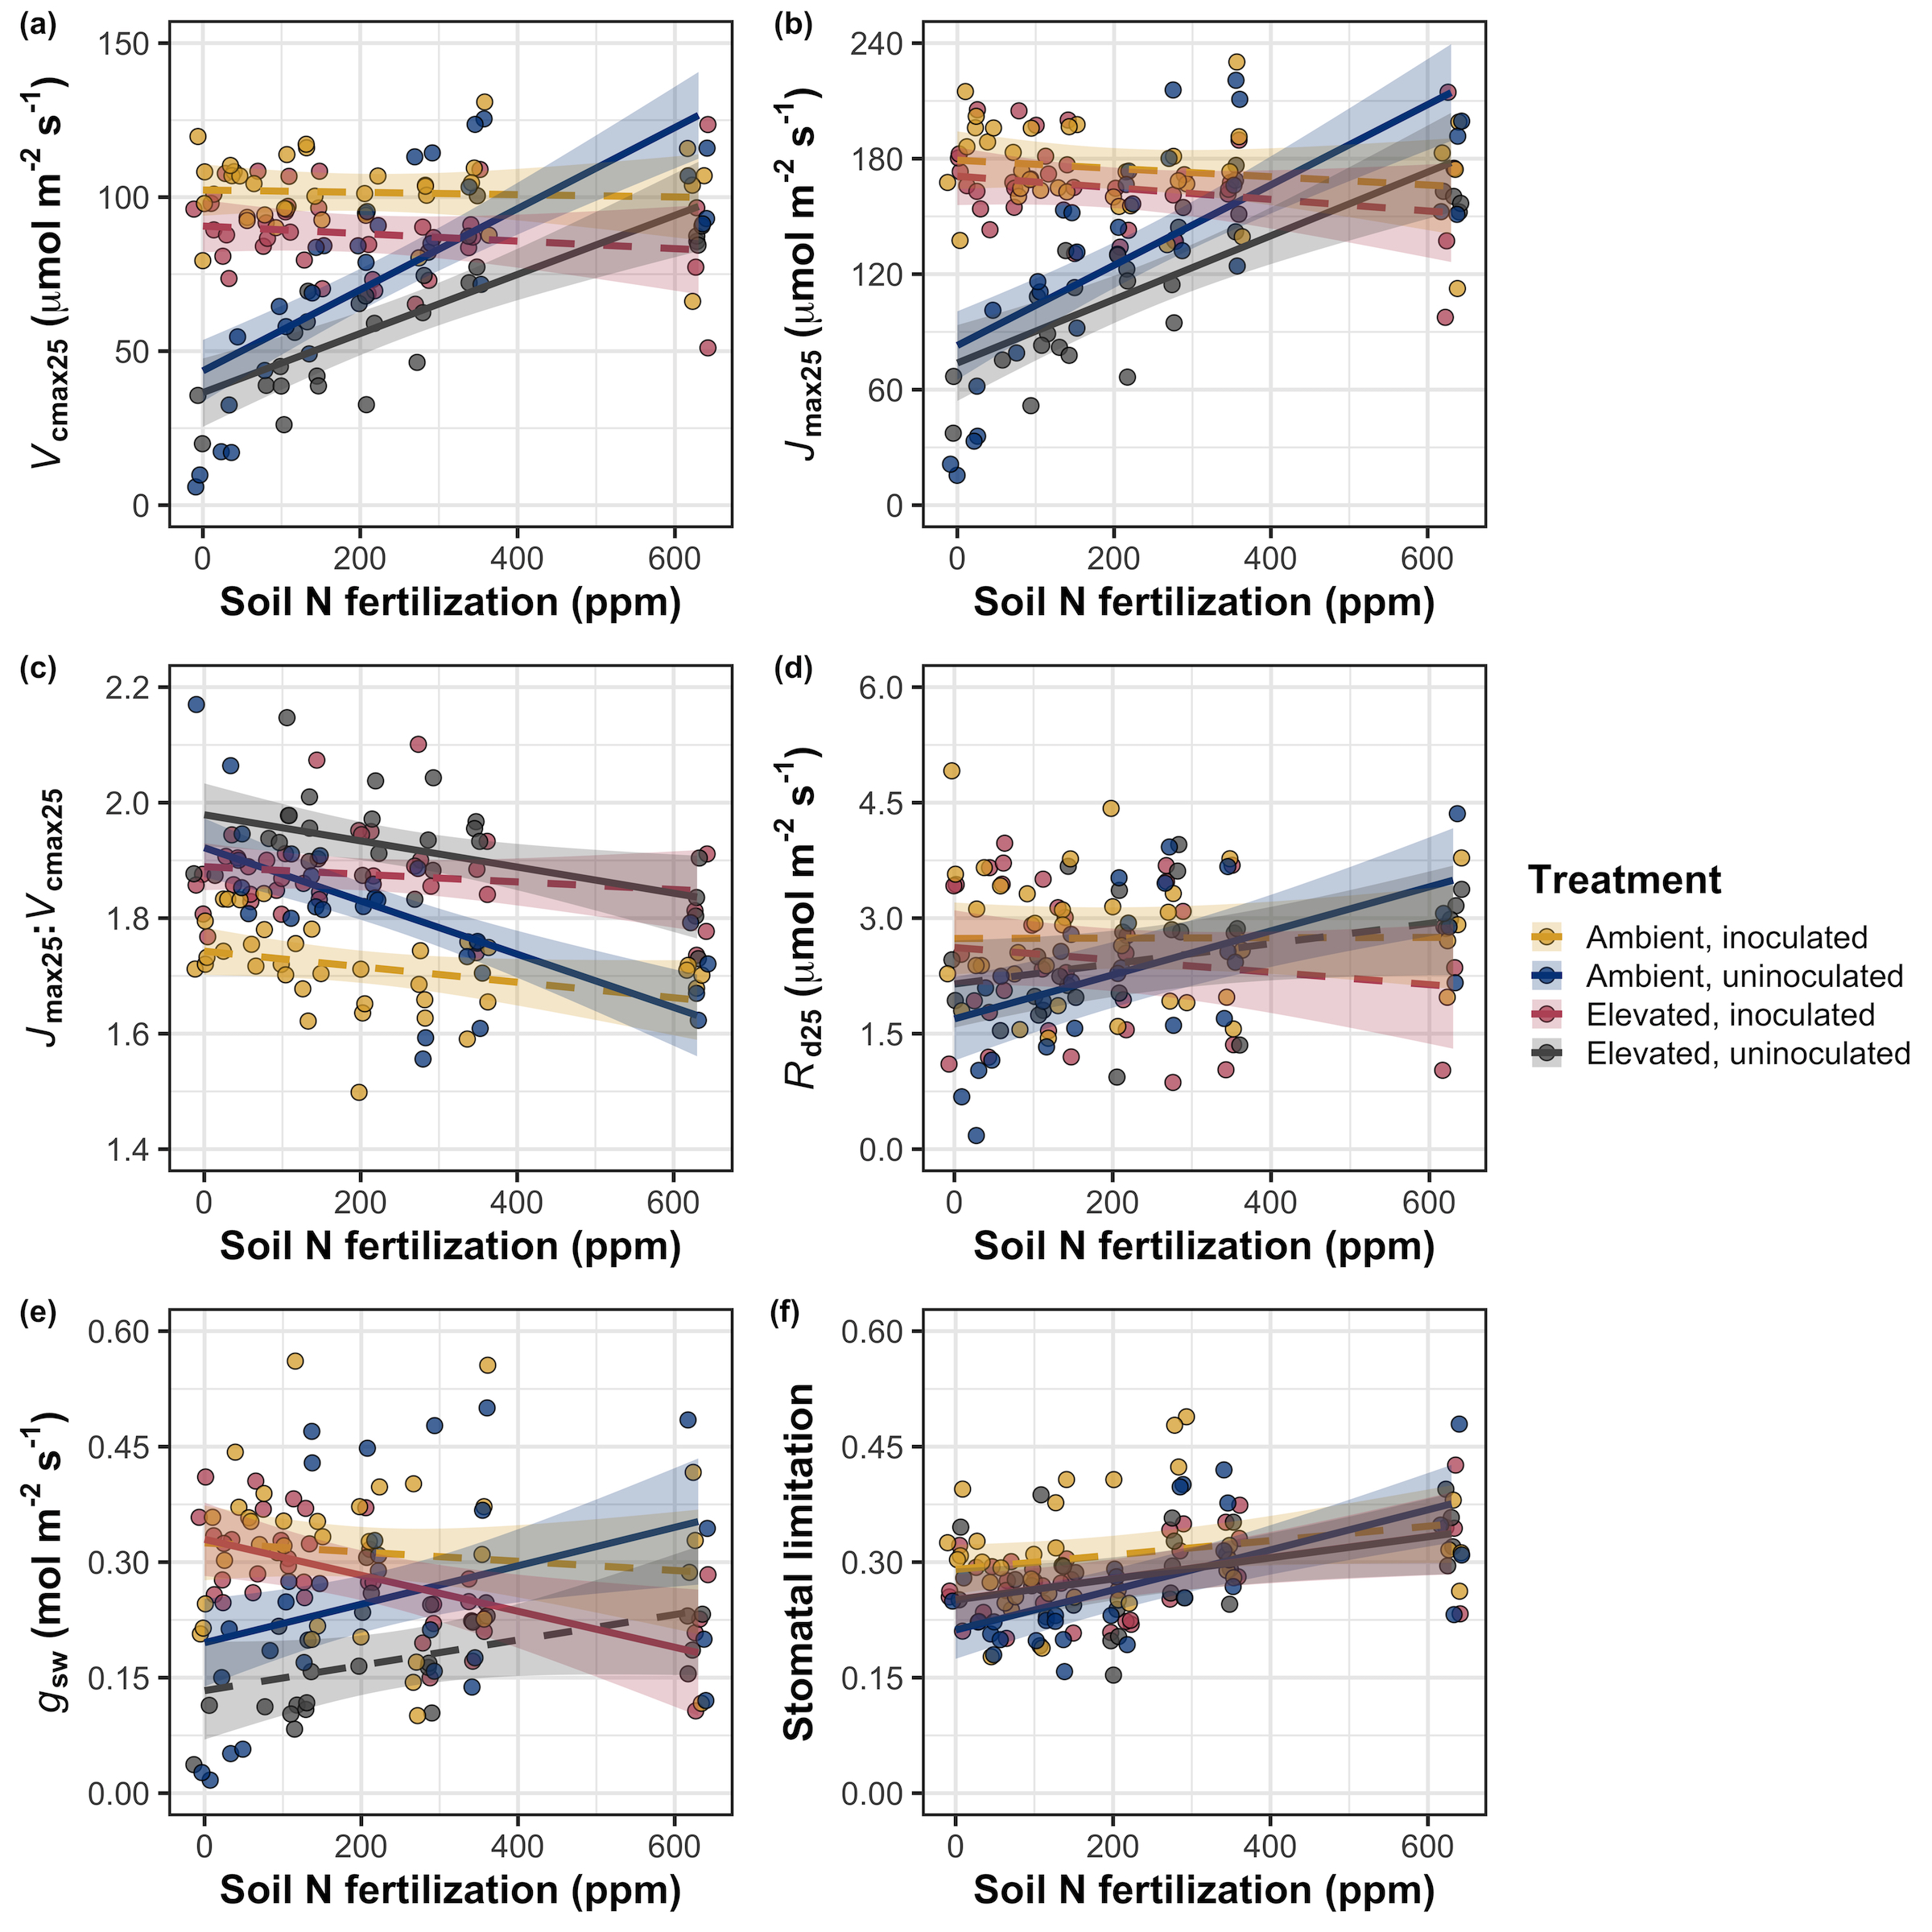
\includegraphics[scale = 0.057]{ch5_NxCO2xI/figs/NxCO2xI_fig2_photo.png}
    \caption[Effects of CO$_2$, fertilization, and inoculation on maximum rate of Rubisco carboxylation, the maximum rate of RuBP regeneration, and the ratio of the maximum rate of RuBP regeneration to the maximum rate of Rubisco carboxylation leaf mass per unit leaf area, dark respiration, stomatal conductance, and stomatal limitation.]{Effects of CO$_2$, fertilization, and inoculation on maximum rate of Rubisco carboxylation (a), the maximum rate of RuBP regeneration (b), and the ratio of the maximum rate of RuBP regeneration to the maximum rate of Rubisco carboxylation leaf mass per unit leaf area (c), dark respiration (d), stomatal conductance (e), and stomatal limitation (f). Soil nitrogen fertilization is represented on the x-axis in all panels. Colored points and trendlines are as explained in Figure 1.}
    \label{fig:figure5.2}
\end{figure}
\clearpage

\subsection{\textit{Leaf nitrogen allocation}}
A relatively stronger downregulation in $N_\mathrm{area}$ than $V_\mathrm{cmax25}$ or $J_\mathrm{max25}$ resulted in an 20\% and 29\% respective stimulation in $\rho_\mathrm{rubisco}$ and $\rho_\mathrm{bioe}$ under elevated CO$_2$ (\textit{p} < 0.001 in both cases; Table 3). There was no apparent CO$_2$ effect on $\rho_\mathrm{light}$ (\textit{p} = 0.700; Table 3), but the strong stimulation in $\rho_\mathrm{rubisco}$ and $\rho_\mathrm{bioe}$ resulted in a 21\% stimulation of $\rho_\mathrm{photo}$ under elevated CO$_2$ (\textit{p} < 0.001; Table 3; Fig. 3A). The stimulation of $\rho_\mathrm{rubisco}$, $\rho_\mathrm{bioe}$, and $\rho_\mathrm{photo}$ due to elevated CO$_2$ was not modified across the fertilization gradient (CO$_2$-by-fertilization interaction: $p_\mathrm{rubisco}$ = 0.269, $p_\mathrm{bioe}$ = 0.298, $p_\mathrm{photo}$ = 0.281; Table 3). A marginal interaction between inoculation and CO2 on $\rho_\mathrm{rubisco}$ and $\rho_\mathrm{photo}$ (CO$_2$-by-inoculation interaction: $p_\mathrm{rubisco}$ = 0.057, $p_\mathrm{photo}$ = 0.057; Table 3) indicated that the general positive effect of inoculation on $\rho_\mathrm{rubisco}$ and $\rho_\mathrm{photo}$ (\textit{p} < 0.001 in both cases; Table 3) was only apparent under ambient CO$_2$ (Tukey: \textit{p} < 0.001 in both cases), with no apparent effect of inoculation under elevated CO$_2$ (Tukey\textsubscript{rubisco}: \textit{p} = 0.200; Tukey\textsubscript{photo}: \textit{p} = 0.147). Inoculation did not modify the stimulation of $\rho_\mathrm{bioe}$ under elevated CO$_2$ (CO$_2$-by-inoculation interaction: \textit{p} = 0.122; Table 3) or the null effect of CO$_2$ on $\rho_\mathrm{bioe}$ (CO$_2$-by-inoculation interaction: \textit{p} = 0.298; Table 3). Strong interactions between fertilization and inoculation on $\rho_\mathrm{rubisco}$, $\rho_\mathrm{bioe}$, and $\rho_\mathrm{photo}$ (fertilization-by-inoculation interaction: \textit{p} < 0.001 in all cases; Table 3) indicated that the general negative effect of increasing fertilization (\textit{p} < 0.001 in all cases; Table 3) was only observed in inoculated pots (Tukey: \textit{p} < 0.001 in all cases), with no apparent effect of fertilization on $\rho_\mathrm{rubisco}$ (Tukey: \textit{p} = 0.612), $\rho_\mathrm{bioe}$ (Tukey: p = 0.544), or $\rho_\mathrm{photo}$ (Tukey: \textit{p} = 0.521; Fig 3B) in uninoculated pots. An additional interaction between fertilization and inoculation on $\rho_\mathrm{light}$ (fertilization-by-inoculation interaction: \textit{p} < 0.001; Table 3) indicated a negative effect of increasing fertilization on $\rho_\mathrm{light}$ in inoculated pots (Tukey: \textit{p} = 0.041), but a positive effect of increasing fertilization in uninoculated pots (Tukey: \textit{p} < 0.001).

The stimulation in $M_\mathrm{area}$ resulted in an 133\% stimulation of $\rho_\mathrm{structure}$ under elevated CO$_2$ (\textit{p} < 0.001; Table 3; Fig 3C). An interaction between fertilization and CO$_2$ (CO$_2$-by-fertilization interaction: \textit{p} = 0.039; Table 3) indicated that the general negative effect of increasing fertilization (p < 0.001; Table 3) on $\rho_\mathrm{structure}$ was marginally stronger under ambient CO$_2$ (Tukey: \textit{p} = 0.055), resulting in a stronger stimulation in $\rho_\mathrm{structure}$ under elevated CO$_2$ with increasing fertilization. A marginal interaction between inoculation and CO$_2$ (CO$_2$-by-inoculation interaction: \textit{p} = 0.057; Table 3) indicated that the general positive effect of inoculation on $\rho_\mathrm{structure}$ (\textit{p} < 0.001; Table 3) was only observed under elevated CO$_2$ (Tukey: \textit{p} < 0.001), with no apparent inoculation effect observed under ambient CO$_2$ (Tukey: \textit{p} = 0.513). Finally, an interaction between fertilization and inoculation (fertilization-by-inoculation interaction: \textit{p} < 0.001; Table 3; Fig. 3D) indicated that, while increasing fertilization generally increased $\rho_\mathrm{structure}$ (\textit{p} < 0.001; Table 3), this response was generally stronger in uninoculated pots (Tukey: \textit{p} = 0.001).

\newpage
placeholder Table 3
\clearpage

\newpage
\begin{landscape}
    \begin{figure}
        \centering
        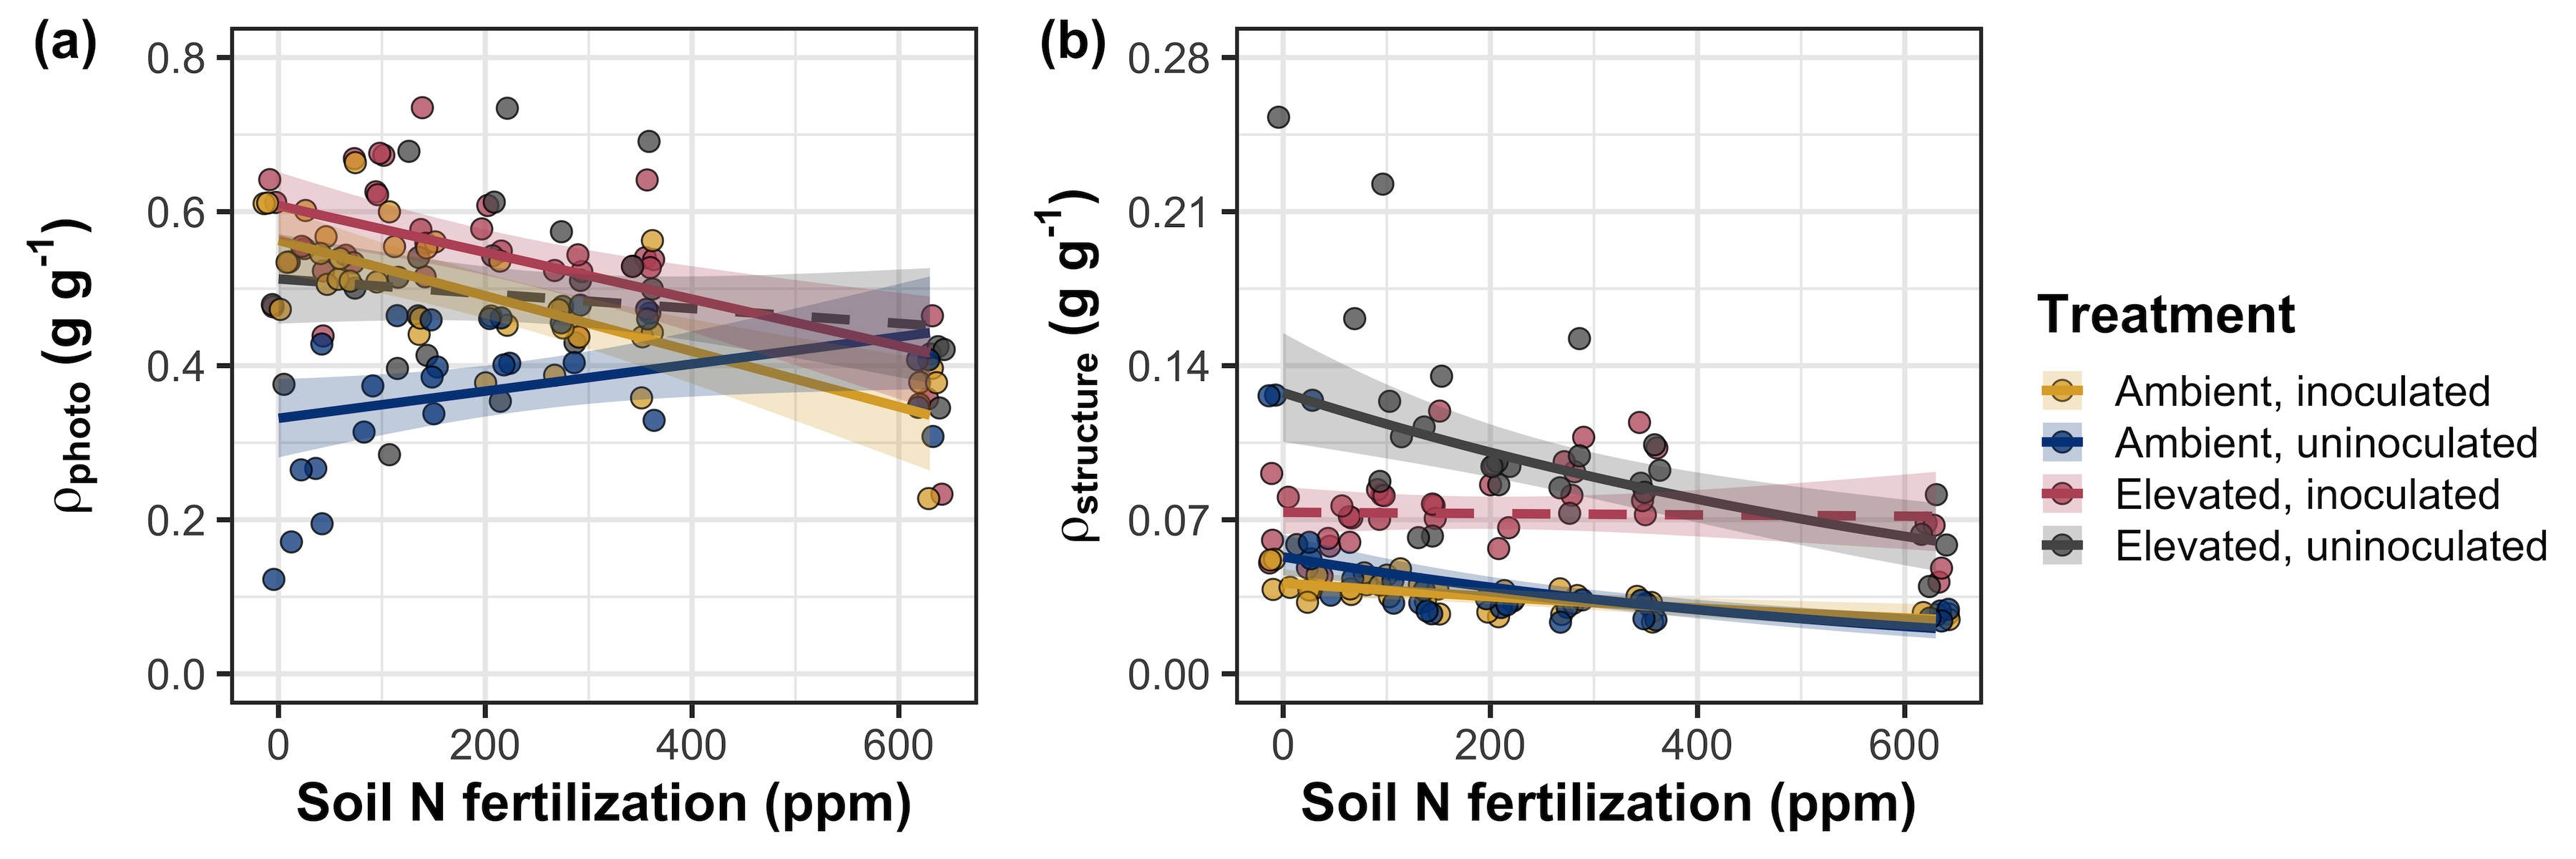
\includegraphics[scale = 0.075]{ch5_NxCO2xI/figs/NxCO2xI_fig3_propN.png}
        \caption[Effects of CO$_2$, fertilization, and inoculation on the relative fraction of leaf nitrogen allocated to photosynthesis and the fraction of leaf nitrogen allocated to structure.]{Effects of CO$_2$, fertilization, and inoculation on the relative fraction of leaf nitrogen allocated to photosynthesis (a) and the fraction of leaf nitrogen allocated to structure (b). Soil nitrogen fertilization is represented on the x-axis in both panels. Colored points and trendlines are as explained in Figure 1.}
        \label{fig:figure5.3}
    \end{figure}
\end{landscape}
\clearpage

\subsection{\textit{Whole plant growth and total leaf area}}
Total leaf area was 51\% greater and total biomass was 102\% greater under elevated CO$_2$ (\textit{p} < 0.001 in both cases; Table 4), a pattern that was enhanced by fertilization (CO$_2$-by-fertilization interaction: \textit{p} < 0.001 in both cases; Table 4; Fig. 4a-b) but was not modified across inoculation treatments (CO$_2$-by-inoculation interaction: $p_{total\_leaf\_area}$ = 0.151, $p_{total\_biomass}$: 0.472; Table 4). Specifically, the general positive effect of increasing fertilization on total leaf area and whole plant biomass (\textit{p} < 0.001 in both cases; Table 4) was stronger under elevated CO$_2$ (Tukey: \textit{p} < 0.001 in both cases). The general positive effect of increasing fertilization on total leaf area was modified by inoculation treatment (fertilization-by-inoculation interaction: \textit{p} < 0.001 in both cases; Table 4), indicating a stronger positive effect of increasing fertilization in uninoculated pots (Tukey: $p_{total\_leaf\_area}$ = 0.002, $p_{total\_biomass}$ = 0.001).

\subsection{\textit{Carbon costs to acquire nitrogen}}
A general 62\% stimulation in $N_\mathrm{cost}$ under elevated CO$_2$ was modified thr-ough a strong three-way interaction between CO$_2$, fertilization, and inoculation (CO$_2$-by-inoculation-by-fertilization interaction: \textit{p} < 0.001; Table 4). This interaction revealed a general negative effect of increasing fertilization on $N_\mathrm{cost}$ (\textit{p} < 0.001; Table 4) that was observed in all treatment combinations (Tukey: \textit{p} < 0.001 in all cases) except for inoculated pots grown under elevated CO$_2$ (Tukey: \textit{p} = 0.779; Fig. 5c). This response also resulted in generally stronger negative effects of increasing fertilization on $N_\mathrm{cost}$ in uninoculated pots grown under elevated CO$_2$ than uninoculated pots grown under ambient CO$_2$ (Tukey: \textit{p} = 0.001) and inoculated pots grown under either ambient CO$_2$ (Tukey: \textit{p} < 0.001) or elevated CO$_2$ (Tukey: \textit{p} < 0.001), while uninoculated pots grown under ambient CO$_2$ had generally stronger negative effects of increasing fertilization on $N_\mathrm{cost}$ than inoculated pots grown under elevated CO$_2$ (Tukey: \textit{p} = 0.002), but not inoculated pots grown under ambient CO$_2$ (Tukey: \textit{p} = 0.216). The general reduction in $N_\mathrm{cost}$ with increasing fertilization and in uninoculated pots were driven by a stronger positive effect of increasing fertilization on $N_\mathrm{wp}$ (denominator of $N_\mathrm{cost}$) than $C_\mathrm{bg}$ (numerator of $N_\mathrm{cost}$), while the general stimulation in $N_\mathrm{cost}$ under elevated CO$_2$ was driven by a stronger positive effect of elevated CO$_2$ on $C_\mathrm{bg}$ than $N_\mathrm{wp}$ (Table 4).

\newpage
placeholder Table 4
\clearpage

\newpage
\begin{figure}
    \centering
    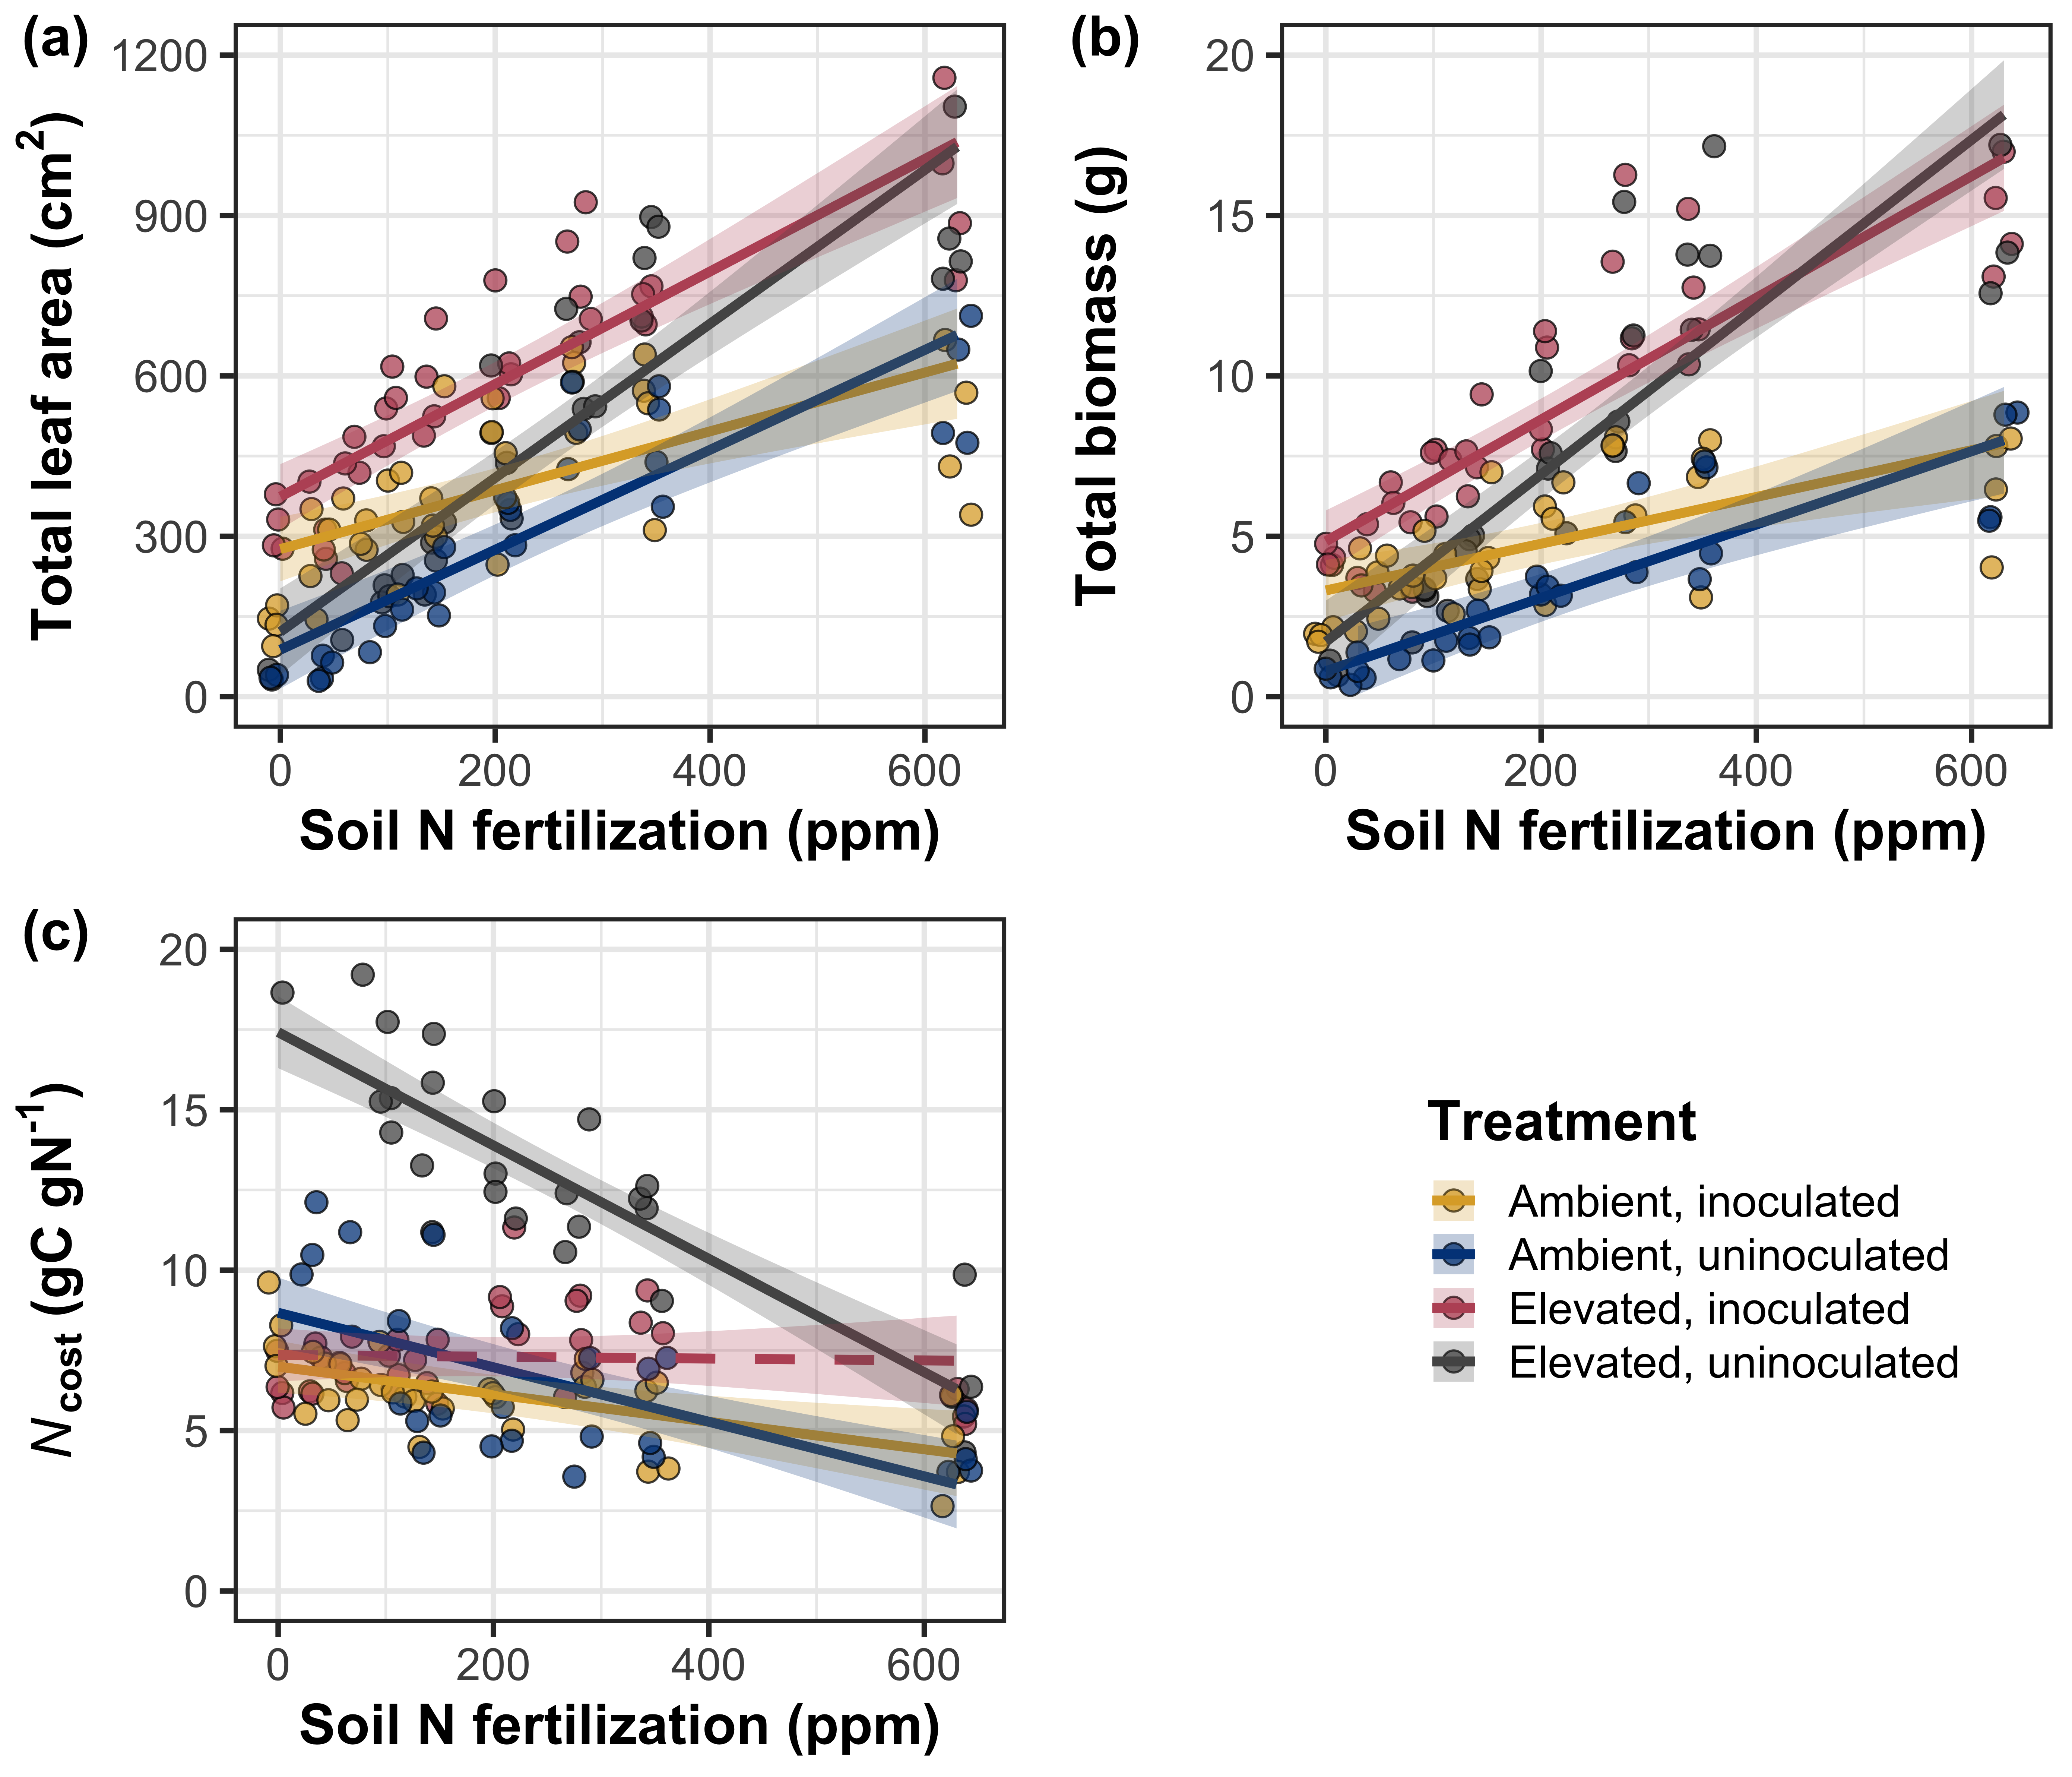
\includegraphics[scale = 0.075]{ch5_NxCO2xI/figs/NxCO2xI_fig4_wholePlant.png}
    \caption[Effects of CO$_2$, fertilization, and inoculation on total leaf area, total biomass, and structural carbon costs to acquire nitrogen.]{Effects of CO$_2$, fertilization, and inoculation on total leaf area (a), total biomass (b), and structural carbon costs to acquire nitrogen (c). Soil nitrogen fertilization is represented continuously on the x-axis in all panels. Colored points and trendlines are as explained in Figure 1.}
    \label{fig:figure5.4}
\end{figure}
\clearpage

\subsection{\textit{Nitrogen fixation}}
Nodule biomass was stimulated by 30\% under elevated CO$_2$ (\textit{p} < 0.001; Table 5), a pattern that was modified across the fertilization gradient (CO$_2$-by-fertilization interaction: \textit{p} = 0.479; Table 5), but not between inoculation treatments (CO$_2$-by-inoculation interaction: p = 0.404; Table 5). Specifically, the general negative effect of increasing fertilization on nodule biomass (\textit{p} < 0.001; Table 5) was stronger under elevated CO$_2$ than ambient CO$_2$ (Tukey: \textit{p} < 0.001; Fig. 5a), which reduced the stimulation in nodule biomass under elevated CO$_2$ with increasing fertilization. A strong interaction between fertilization and inoculation (fertilization-by-inoculation interaction: \textit{p} < 0.001; Table 5) was driven by a stronger negative effect of increasing fertilization in inoculated pots (Tukey: \textit{p} < 0.001; Fig. 5a).

There was no effect of CO$_2$ on nodule: root biomass (\textit{p} = 0.767; Table 5), although an interaction between CO$_2$ and inoculation (CO$_2$-by-inoculation interaction: \textit{p} < 0.001; Table 5) indicated that the general positive effect of inoculation on nodule: root biomass (\textit{p} < 0.001; Table 5) was stronger under ambient CO$_2$ (3129\% increase; Tukey: \textit{p} < 0.001) than elevated CO$_2$ (379\% increase; Tukey: \textit{p} < 0.001; Fig. 5b). The null effect of CO$_2$ on nodule: root biomass was consistently observed across the fertilization gradient (\textit{p} = 0.183; Table 5; Fig. 5b). An interaction between fertilization and inoculation (fertilization-by-inoculation interaction: \textit{p} < 0.001; Table 5) indicated that the general negative effect of increasing fertilization on nodule: root biomass (\textit{p} < 0.001; Table 5) was stronger in inoculated pots (Tukey: \textit{p} < 0.001; Fig. 5b). 

There was no effect of CO$_2$ on \%$N_\mathrm{dfa}$ (\textit{p} = 0.472; Table 5), a pattern that was not modified by inoculation (CO$_2$-by-inoculation interaction: \textit{p} = 0.156; Table 5) or fertilization (CO$_2$-by-fertilization interaction: \textit{p} = 0.099; Table 5). An interaction between fertilization and inoculation (fertilization-by-inoculation interaction: \textit{p} < 0.001; Table 5) indicated that the general negative effect of increasing fertilization on \%Ndfa (\textit{p} < 0.001; Table 5) was only observed in inoculated pots (Tukey: \textit{p} < 0.001), with no apparent effect of fertilization on \%$N_\mathrm{dfa}$ in uninoculated pots (Tukey: \textit{p} = 0.651; Table 5; Fig. 5c).

\newpage
placeholder Table 5
\clearpage

\newpage
\begin{figure}
    \centering
    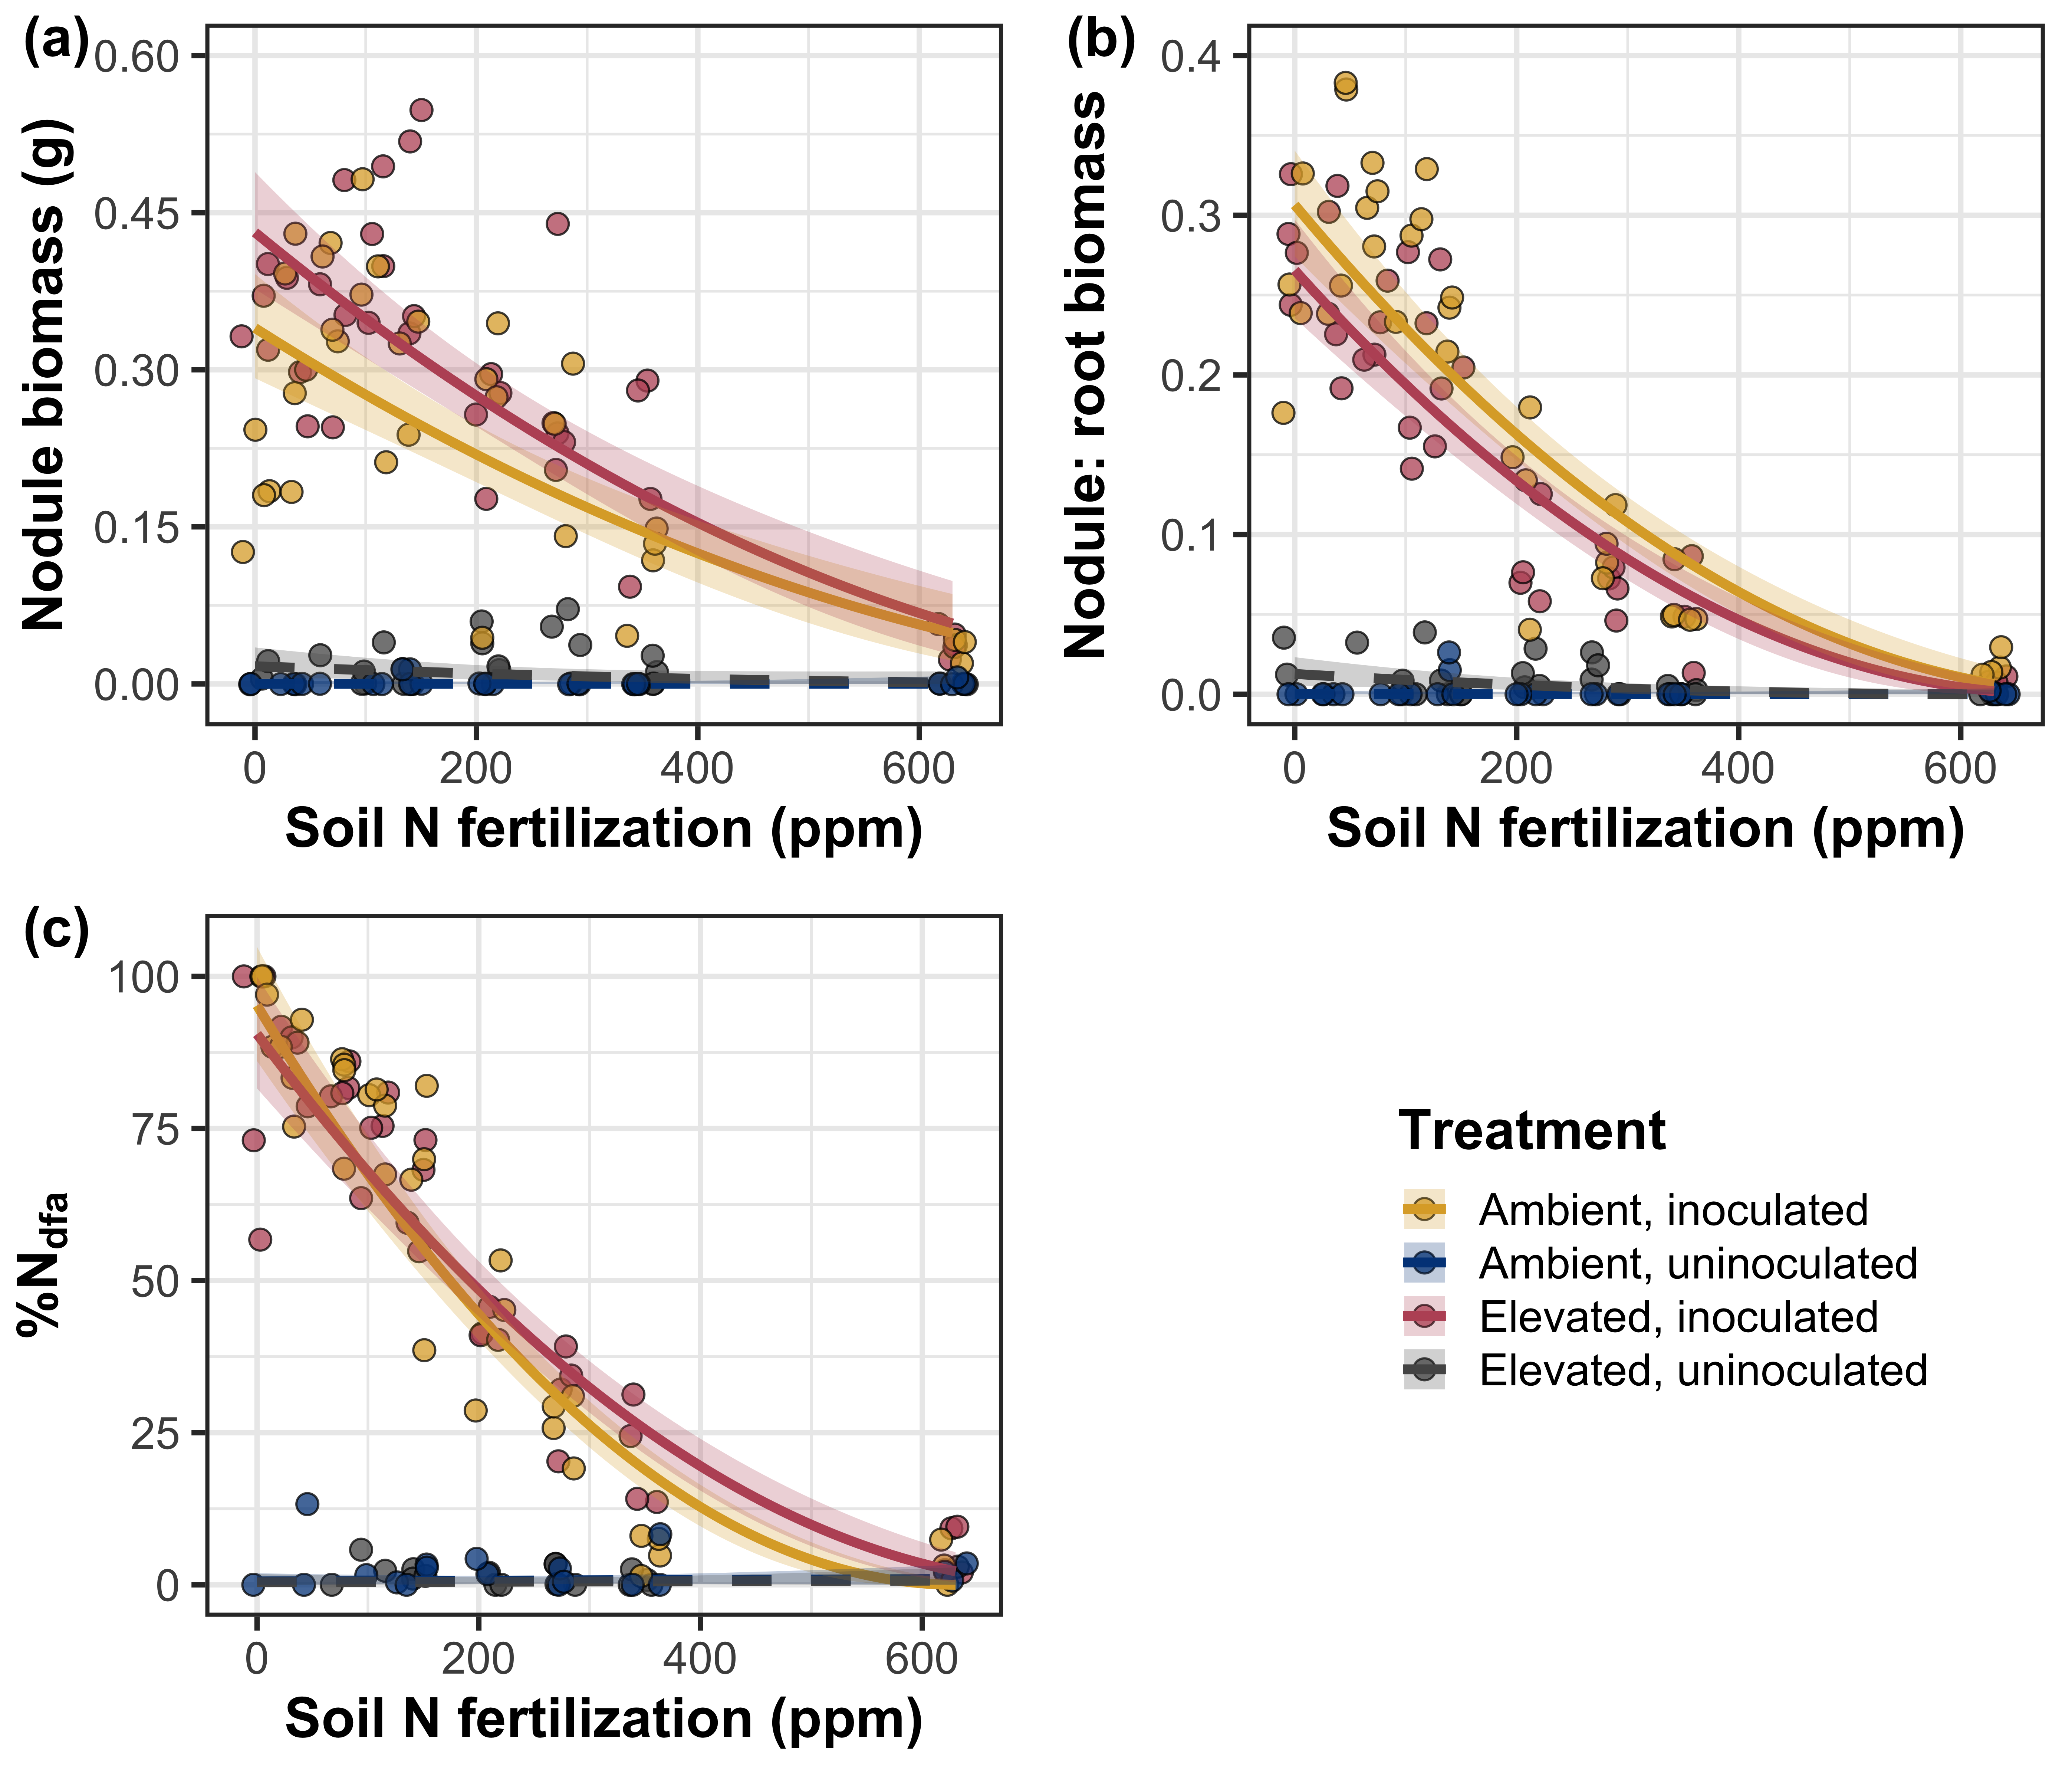
\includegraphics[scale = 0.075]{ch5_NxCO2xI/figs/NxCO2xI_fig5_nFix.png}
    \caption[Effects of CO$_2$, fertilization, and inoculation on nodule biomass, nodule: root biomass, and percent nitrogen fixed from the atmosphere.]{Effects of CO$_2$, fertilization, and inoculation on nodule biomass (a), nodule: root biomass (b), and percent nitrogen fixed from the atmosphere (c). Soil nitrogen fertilization is represented on the x-axis. Yellow points and trendlines indicate inoculated individuals grown under ambient CO$_2$, blue points and trendlines indicate uninoculated individuals grown under ambient CO$_2$, red points and trendlines indicate inoculated individuals grown under elevated CO$_2$, and grey points indicate uninoculated individuals grown under elevated CO$_2$. Solid trendlines indicate slopes that are different from zero (\textit{p} < 0.05), while dashed trendlines indicate slopes that are not different from zero (\textit{p} > 0.05). Curvilinear trendlines occur as a result of back-transforming models where response variables received either a natural log or square root transformation prior to fitting. }
    \label{fig:figure5.5}
\end{figure}
\clearpage

\section{Discussion}

In this study, we determined leaf and whole plant acclimation responses of 7-week \textit{G. max} seedlings grown under two CO$_2$ concentrations, two inoculation treatments, and nine soil nitrogen fertilization treatments in a full-factorial growth chamber experiment. In support of our hypotheses and patterns expected from theory, elevated CO$_2$ reduced $N_\mathrm{area}$, $V_\mathrm{cmax25}$, and $J_\mathrm{max25}$. The relatively stronger downregulation in $V_\mathrm{cmax25}$ than $J_\mathrm{max25}$ under elevated CO$_2$ resulted in a stimulation in $J_\mathrm{max25}$:$V_\mathrm{cmax25}$ under elevated CO$_2$. The downregulation of $V_\mathrm{cmax25}$ and $J_\mathrm{max25}$ under elevated CO$_2$ was similar across fertilization and inoculation treatments, indicating that the CO$_2$ responses were not due to nitrogen limitation. Interestingly, our results indicate that elevated CO$_2$ increased the fraction of leaf nitrogen allocated to photosynthesis and structure, leading to a stimulation in nitrogen use efficiency under elevated CO$_2$ despite the apparent downregulation in $N_\mathrm{area}$, $V_\mathrm{cmax25}$, and $J_\mathrm{max25}$. The downregulation in leaf photosynthetic processes under elevated CO$_2$ also corresponded with a strong stimulation in total leaf area and total biomass. Strong stimulations in whole plant growth due to elevated CO$_2$ were generally enhanced with increasing fertilization and were negatively related to structural carbon costs to acquire nitrogen. Inoculation generally did not modify whole plant responses to elevated CO$_2$ across the fertilization gradient, likely due to a strong reduction in root nodulation with increasing fertilization. However, strong positive effects of inoculation on whole plant growth were observed under low fertilization, consistent with our hypothesis. Overall, observed leaf and whole plant acclimation responses to CO$_2$ support our hypotheses and patterns expected from photosynthetic least-cost theory, showing that leaf acclimation responses to CO$_2$ were decoupled from soil nitrogen availability and ability to acquire nitrogen via symbiotic nitrogen fixation. Instead, leaf acclimation responses were driven by optimal resource investment to photosynthetic capacity, which maximized nitrogen allocation to structures that support whole plant growth.